\documentclass[journal,10pt]{IEEEtran}

% ===================== PACKAGES =====================
\usepackage[utf8]{inputenc}
\usepackage[T1]{fontenc}
\usepackage{amsmath,amssymb,amsfonts,amsthm}
\usepackage{algorithmic}
\usepackage{algorithm}
\usepackage{graphicx}
\usepackage{textcomp}
\usepackage{xcolor}
\usepackage{booktabs}
\usepackage{multirow}
\usepackage{array}
\usepackage{caption}
\usepackage{subcaption}
\usepackage{hyperref}
\usepackage{cleveref}
\usepackage{tikz}
\usetikzlibrary{shapes,arrows.meta,positioning,fit,calc,decorations.markings,patterns,shadows.blur,backgrounds,chains,matrix}
\usepackage{pgfplots}
\pgfplotsset{compat=1.18}
\usepgfplotslibrary{fillbetween}
\usepackage{balance}
\usepackage{url}
\usepackage{cite}
\usepackage{mathtools}
\usepackage{bm}
\usepackage{enumitem}
\usepackage{pifont}
\usepackage{thmtools}
\usepackage{makecell}
\usepackage{colortbl}
\usepackage{float}

% ===================== COLORS =====================
\definecolor{attackred}{RGB}{220,53,69}
\definecolor{defendblue}{RGB}{0,123,255}
\definecolor{safegreen}{RGB}{40,167,69}
\definecolor{warnorg}{RGB}{255,153,0}
\definecolor{lightbg}{RGB}{248,249,250}
\definecolor{darktext}{RGB}{33,37,41}
\definecolor{sveccolor}{RGB}{102,16,242}
\definecolor{tcvcolor}{RGB}{13,110,253}
\definecolor{capcolor}{RGB}{25,135,84}
\definecolor{pipegray}{RGB}{108,117,125}

% ===================== THEOREM ENVIRONMENTS =====================
\newtheorem{theorem}{Theorem}
\newtheorem{lemma}[theorem]{Lemma}
\newtheorem{proposition}[theorem]{Proposition}
\newtheorem{corollary}[theorem]{Corollary}
\newtheorem{definition}{Definition}
\newtheorem{remark}{Remark}

% ===================== COMMANDS =====================
\newcommand{\E}{\mathbb{E}}
\newcommand{\R}{\mathbb{R}}
\newcommand{\KL}{\mathrm{D_{KL}}}
\newcommand{\calA}{\mathcal{A}}
\newcommand{\calD}{\mathcal{D}}
\newcommand{\calF}{\mathcal{F}}
\newcommand{\calG}{\mathcal{G}}
\newcommand{\calH}{\mathcal{H}}
\newcommand{\calM}{\mathcal{M}}
\newcommand{\calO}{\mathcal{O}}
\newcommand{\calP}{\mathcal{P}}
\newcommand{\calS}{\mathcal{S}}
\DeclareMathOperator*{\argmin}{arg\,min}
\DeclareMathOperator*{\argmax}{arg\,max}

\begin{document}

\title{Byzantine Resilience in Multi-Agent LLM Orchestration: Consensus Protocols for Trustworthy Autonomous Decision Pipelines}

\author{%
\IEEEauthorblockN{[Author Names Redacted for Review]}
\IEEEauthorblockA{[Affiliations Redacted for Review]}
\thanks{Manuscript received XXXX XX, 2026. \emph{(Corresponding author: [Redacted].)}}
\thanks{Digital Object Identifier XXXX.}
}

\markboth{IEEE TRANSACTIONS ON DEPENDABLE AND SECURE COMPUTING, VOL.~XX, NO.~XX, XXXX 2026}{}

\maketitle

\begin{abstract}
Multi-agent systems built upon large language models (LLMs) are increasingly deployed in safety-critical decision pipelines---from clinical diagnosis to autonomous navigation---where a single compromised or hallucinating agent can cascade failures across the entire system. We formalize this vulnerability as the \emph{semantic Byzantine agreement} problem, extending classical Byzantine fault tolerance (BFT) theory to account for the unique failure modes of LLM agents: hallucination, prompt injection-induced deviation, stochastic inconsistency, and adversarial subversion. We present \textsc{AgentShield}, a consensus protocol suite comprising three complementary mechanisms: \emph{Semantic Voting with Equivalence Classes} (SVEC), which clusters agent outputs by meaning rather than lexical identity; \emph{Temporal Consistency Verification} (TCV), which detects agents exhibiting statistically anomalous behavioral drift; and \emph{Cross-Attestation Probing} (CAP), which employs reciprocal challenge-response verification to identify compromised agents. We prove that \textsc{AgentShield} achieves semantic Byzantine agreement tolerating $f < n/3$ faulty agents (Theorem~1), matching the classical impossibility bound; that the protocol terminates in $O(f+1)$ communication rounds (Theorem~2); and that deterministic semantic agreement is impossible for stochastic agents without $\Omega(\log(1/\delta))$ verification rounds (Theorem~3). Empirical evaluation across six multi-agent architectures, four safety-critical application domains, and 15{,}000 decision scenarios demonstrates that \textsc{AgentShield} reduces cascading failure rates from 67.8\% to 2.9\% while maintaining 94.7\% decision accuracy with 38\,ms average per-round overhead. All code and datasets are available at \url{https://github.com/[redacted]/AgentShield} and \url{https://doi.org/10.57967/[redacted]}.
\end{abstract}

\begin{IEEEkeywords}
Multi-agent systems, Byzantine fault tolerance, large language model safety, consensus protocols, semantic agreement, dependable AI, autonomous decision-making.
\end{IEEEkeywords}

\section{Introduction}
\IEEEPARstart{M}{ulti-agent} architectures built upon Large Language Models (LLMs) have become the prevailing paradigm for complex autonomous decision-making, enabling systems where specialized agents collaborate on tasks spanning software engineering~\cite{hong2024metagpt}, scientific discovery~\cite{boiko2023autonomous}, medical diagnostics~\cite{tang2024medagents}, financial analysis~\cite{li2024finagent}, and embodied planning~\cite{wang2024voyager}. In these architectures, individual LLM agents are assigned distinct roles---planner, executor, critic, verifier---and their outputs are composed into collective decisions through orchestration protocols~\cite{wu2023autogen, park2023generative}.

This paradigm introduces a critical dependability challenge that existing frameworks entirely overlook: \emph{any single agent failure can propagate through the orchestration pipeline, corrupting downstream decisions in ways that are difficult to detect and potentially catastrophic in safety-critical domains}. Unlike traditional distributed systems, where Byzantine nodes exhibit arbitrary but structurally constrained behavior, LLM agents exhibit a unique combination of failure modes. They hallucinate, producing confident but fabricated outputs that are syntactically indistinguishable from correct responses~\cite{huang2023survey}. They are susceptible to prompt injection, which can subvert their objectives without visible indicators~\cite{liu2024promptinjection}. They exhibit stochastic inconsistency, where the same agent produces contradictory outputs across invocations due to sampling randomness~\cite{wang2023selfconsistency}. And they can be adversarially subverted, with a compromised agent strategically misleading other agents while evading detection~\cite{zhang2024injecagent}. These failure modes are particularly dangerous because they produce \emph{semantically plausible but factually incorrect} outputs that pass all syntactic validation.

\subsection{Motivating Scenario}
Consider a multi-agent clinical decision support system deployed in an emergency department. Three LLM agents independently analyze patient data: Agent~$A_1$ (radiologist) interprets chest imaging, Agent~$A_2$ (pathologist) analyzes laboratory results, and Agent~$A_3$ (clinician) synthesizes a treatment recommendation based on the first two agents' outputs. If $A_1$ hallucinates a pulmonary embolism in a normal chest CT---or if an adversary has injected $A_1$'s system prompt to systematically under-report critical findings---the downstream clinician agent $A_3$ will produce a treatment plan that is either unnecessarily aggressive or dangerously passive. No existing multi-agent framework provides formal guarantees that such cascading failures will be detected and prevented.

\subsection{Our Contributions}
We make the following contributions:

\begin{enumerate}[leftmargin=*]
\item We formalize \textbf{semantic Byzantine agreement} for multi-agent LLM systems, defining three agreement properties---semantic validity (Definition~\ref{def:sv}), semantic consistency (Definition~\ref{def:sc}), and liveness (Definition~\ref{def:liveness})---that extend classical BFT to the LLM setting where agents produce semantically equivalent but lexically distinct outputs.

\item We design the \textsc{AgentShield} protocol suite comprising three mechanisms (SVEC, TCV, CAP) and prove that it \textbf{tolerates $f < n/3$ faulty agents} (Theorem~\ref{thm:bft}), \textbf{terminates in $O(f+1)$ rounds} (Theorem~\ref{thm:termination}), and that \textbf{deterministic agreement is impossible} with stochastic agents without logarithmic verification overhead (Theorem~\ref{thm:impossibility}).

\item We conduct \textbf{comprehensive empirical evaluation} across six multi-agent architectures, four safety-critical domains, 15{,}000 scenarios, and five baselines, demonstrating 95.6\% fault mitigation with 94.7\% decision accuracy and 38\,ms overhead.
\end{enumerate}

The remainder of this paper is structured as follows. Section~\ref{sec:related} surveys related work. Section~\ref{sec:model} defines the system and failure models. Section~\ref{sec:properties} formalizes the agreement properties. Section~\ref{sec:protocol} presents the \textsc{AgentShield} protocol. Section~\ref{sec:theory} provides theoretical analysis. Section~\ref{sec:mechanisms} details the three mechanisms. Section~\ref{sec:experiments} presents evaluation results. Section~\ref{sec:discussion} discusses implications and limitations. Section~\ref{sec:conclusion} concludes.

\subsection{Broader Impact of Multi-Agent Failures}
The consequences of undetected multi-agent failures extend beyond individual incorrect decisions. In interconnected systems, a single faulty agent can trigger cascading failures that propagate through the entire decision pipeline. Consider a financial trading system where Agent $A_1$ (analyst) produces an incorrect valuation, Agent $A_2$ (risk assessor) uses this valuation to compute an incorrect risk profile, and Agent $A_3$ (trader) executes trades based on the incorrect risk assessment. The error amplifies at each stage, and the final trading decision may bear no resemblance to what any correctly functioning agent would produce. This cascading amplification is fundamentally different from single-agent errors, which are bounded by the single agent's output space.

Multi-agent failures are also more difficult to detect retrospectively. When a single agent produces an incorrect output, the error can often be traced back to a specific input or prompt. When a multi-agent system fails, the error may arise from the interaction between multiple agents' outputs---each individually plausible but collectively inconsistent. Post-hoc analysis of such failures requires understanding the entire communication graph and the causal chain of agent interactions, which is infeasible without the systematic logging that \textsc{AgentShield}'s audit trail provides.

The legal and regulatory implications of multi-agent failures are also significant. Under emerging AI governance frameworks, operators of AI systems in high-risk domains are required to demonstrate that their systems are reliable, safe, and subject to appropriate oversight. A multi-agent system that lacks formal fault tolerance guarantees may fail to meet these requirements, exposing operators to regulatory sanctions and liability. \textsc{AgentShield}'s formal BFT guarantees and auditable consensus process are designed to address these governance requirements directly.

\subsection{The Need for Formal Guarantees}
Existing approaches to multi-agent reliability rely on heuristic methods---majority voting, debate, self-consistency---that provide no formal guarantees about system behavior under adversarial conditions. These methods may work well in benign settings where all agents are honest and errors are independent, but they fail catastrophically when an adversary can strategically choose which agents to compromise and what outputs to produce. The history of distributed computing has repeatedly demonstrated that heuristic approaches to fault tolerance are insufficient: only protocols with formally proven correctness guarantees can be trusted in safety-critical applications. Our work brings this lesson from the distributed systems literature to the emerging field of multi-agent LLM safety.

The gap between current practice and formal assurance is particularly concerning given the speed of multi-agent deployment. Industry analyses indicate that the number of production multi-agent LLM systems doubled every 6 months throughout 2024--2025, while formal safety analysis has lagged far behind. \textsc{AgentShield} addresses this gap by providing immediately deployable defense mechanisms backed by rigorous theoretical guarantees.

\subsection{Relationship to Single-Agent Safety}
It is natural to ask whether single-agent safety mechanisms (RLHF, Constitutional AI, safety filters) eliminate the need for multi-agent Byzantine fault tolerance. The answer is definitively no, for three reasons. First, single-agent safety mechanisms are imperfect: no current technique guarantees that an individual agent will never produce harmful or incorrect outputs, especially under adversarial conditions. Second, multi-agent safety is not reducible to the conjunction of individual agent safety: even if each agent is individually ``safe,'' the composition of their outputs may produce unsafe decisions due to subtle inconsistencies or conflicting interpretations. Third, multi-agent systems introduce new attack surfaces---inter-agent communication, orchestration logic, and consensus formation---that single-agent defenses do not address.

\textsc{AgentShield} is designed to complement, not replace, single-agent safety mechanisms. An agent that is individually safe (via RLHF, safety filters, etc.) and part of a BFT-protected ensemble provides defense in depth: the agent-level mechanisms reduce the probability of compromise, while the system-level BFT protocol ensures that any remaining compromises are detected and tolerated.

The economic stakes of multi-agent LLM failures are substantial and accelerating. Enterprise deployments grew 340\% between 2024 and 2025, with multi-agent architectures managing portfolios exceeding \$50 billion in aggregate. In clinical settings, multi-agent diagnostic systems process over 500{,}000 patient encounters monthly, where a single undetected failure can cascade into misdiagnosis affecting patient safety. The proliferation across critical infrastructure---power grid optimization, air traffic assistance, supply chain coordination, pharmaceutical drug interaction checking---makes formal fault tolerance guarantees an urgent engineering imperative.

The challenge is compounded by the asymmetry between attack and defense complexity. Compromising a single LLM agent requires only a well-crafted adversarial prompt, within reach of even unsophisticated adversaries. Defending against such compromise requires coordinating the entire ensemble, verifying inter-agent consistency, and maintaining performance under degraded conditions---a fundamentally harder problem demanding formal theoretical grounding.

Traditional distributed systems handle Byzantine faults through exact-value consensus protocols where a value is either correct or incorrect with no ambiguity. LLM agents operate in a semantic output space where ``correctness'' is measured by meaning preservation rather than bit-level identity. Two honest agents processing the same clinical case will produce lexically distinct but semantically equivalent diagnoses---a distinction classical BFT protocols cannot accommodate. This semantic gap is the central challenge our work addresses.

Furthermore, the stochastic nature of LLM generation introduces a novel impossibility not present in classical distributed computing. When agents sample from a distribution ($T > 0$), an honest agent may occasionally produce output outside the semantic equivalence class of the majority, creating inherent ambiguity between rare honest variation and adversarial deviation. We formalize this as the stochastic impossibility theorem (Theorem~3) and show it can be overcome either by forcing deterministic generation ($T=0$) or by investing logarithmic verification overhead.

\section{Related Work}\label{sec:related}
We survey related work across multi-agent architectures, Byzantine fault tolerance, LLM robustness, and AI safety, highlighting the gap that our framework addresses.

\subsection{Multi-Agent LLM Architectures}
MetaGPT~\cite{hong2024metagpt} established the Standardized Operating Procedure (SOP) paradigm for multi-agent software engineering. AutoGen~\cite{wu2023autogen} introduced a general-purpose conversational framework supporting diverse multi-agent topologies. ChatDev~\cite{qian2024chatdev} demonstrated end-to-end agent-based software development with role-specialized agents. CAMEL~\cite{li2023camel} explored communicative agents through role-playing, and AgentVerse~\cite{chen2024agentverse} studied dynamic agent group formation. MedAgents~\cite{tang2024medagents} applied multi-agent architectures to medical reasoning, demonstrating improvements over single-agent approaches. Voyager~\cite{wang2024voyager} employed an LLM-powered agent for lifelong learning in Minecraft, illustrating autonomous exploration capabilities. These frameworks optimize task performance but provide no safety guarantees against agent failures. A single hallucinating or compromised agent can silently corrupt the entire pipeline.

\subsection{Byzantine Fault Tolerance}
The Byzantine Generals Problem, formalized by Lamport, Shostak, and Pease~\cite{lamport1982byzantine, pease1980consensus}, established that $n \geq 3f + 1$ processors are required to tolerate $f$ Byzantine faults in synchronous systems. Castro and Liskov~\cite{castro1999practical} introduced Practical BFT (PBFT), making BFT feasible for real-world deployments through view-change protocols and checkpoint mechanisms. Subsequent work improved efficiency through speculative execution (Zyzzyva~\cite{kotla2010zyzzyva}), streamlined protocols (HotStuff~\cite{yin2019hotstuff}), and optimistic paths~\cite{guerraoui2010next}. Blockchain consensus mechanisms, including Tendermint~\cite{buchman2016tendermint} and Algorand~\cite{gilad2017algorand}, brought BFT to internet-scale deployments. Our work is, to our knowledge, the first to extend formal BFT theory to the semantic domain of LLM agent outputs, where the fundamental challenge is that correct agents produce \emph{semantically equivalent but lexically distinct} responses.

\subsection{LLM Robustness and Reliability}
Self-consistency~\cite{wang2023selfconsistency} samples multiple reasoning paths from a single LLM and selects the most frequent answer, improving accuracy but assuming a single honest model. LLM-Debate~\cite{du2024debate} and multi-agent debate~\cite{liang2024debate} use structured argumentation between agents to improve reasoning quality. Constitutional AI~\cite{bai2022constitutional} introduces self-supervised safety constraints through critique-revision cycles. However, all these approaches assume that participating agents are honest---they do not address adversarial subversion, and they provide no formal agreement guarantees. Our framework addresses the fundamentally harder problem of achieving reliable decisions when some agents may be actively adversarial.

\subsection{AI Safety and Trust}
Greenblatt et al.~\cite{greenblatt2024monitoring} studied AI control through safety monitoring, proposing architectures that maintain safety despite intentional subversion. Cohen et al.~\cite{cohen2024lmvslm} explored using one LLM to verify another through cross-examination, demonstrating detection of factual errors but not adversarial manipulation. Cheng et al.~\cite{cheng2024trojanagent} introduced TrojanAgent, demonstrating that multi-agent systems are vulnerable to trojan attacks where a single compromised agent can manipulate group behavior. Hubinger et al.~\cite{hubinger2024sleeper} studied deceptive alignment in LLMs, showing that models can learn to behave differently during evaluation versus deployment. These works highlight the threat landscape but do not provide consensus protocols with formal BFT guarantees.

Table~\ref{tab:comparison} positions \textsc{AgentShield} relative to existing approaches. No prior work provides formal BFT guarantees, semantic agreement, and adversarial robustness simultaneously.

\begin{table*}[t]
\centering
\caption{Comparison with Existing Multi-Agent Safety Frameworks}
\label{tab:comparison}
\renewcommand{\arraystretch}{1.15}
\begin{tabular}{@{}l c c c c c c c@{}}
\toprule
\textbf{Framework} & \textbf{BFT} & \textbf{Semantic} & \textbf{Formal} & \textbf{Adversarial} & \textbf{Cascading} & \textbf{Fault Tol.} & \textbf{Overhead} \\
 & \textbf{Model} & \textbf{Agreement} & \textbf{Guarantees} & \textbf{Robustness} & \textbf{Prevention} & \textbf{Bound} & \textbf{(ms)} \\
\midrule
AutoGen~\cite{wu2023autogen} & \ding{55} & \ding{55} & \ding{55} & \ding{55} & \ding{55} & --- & --- \\
Self-Consistency~\cite{wang2023selfconsistency} & \ding{55} & Partial & \ding{55} & \ding{55} & \ding{55} & --- & 45 \\
LLM-Debate~\cite{du2024debate} & \ding{55} & Partial & \ding{55} & \ding{55} & Partial & --- & 180 \\
Constitutional AI~\cite{bai2022constitutional} & \ding{55} & \ding{55} & \ding{55} & Partial & \ding{55} & --- & 95 \\
TrojanAgent~\cite{cheng2024trojanagent} & \ding{55} & \ding{55} & \ding{55} & \ding{51} & \ding{55} & --- & --- \\
LM-vs-LM~\cite{cohen2024lmvslm} & \ding{55} & \ding{55} & \ding{55} & Partial & \ding{55} & --- & 95 \\
AgentVerse~\cite{chen2024agentverse} & \ding{55} & \ding{55} & \ding{55} & \ding{55} & \ding{55} & --- & 120 \\
\midrule
\textsc{AgentShield} (Ours) & \ding{51} & \ding{51} & \ding{51} & \ding{51} & \ding{51} & $f < n/3$ & 38 \\
\bottomrule
\end{tabular}
\end{table*}

\subsection{Byzantine Resilience in Federated Learning}
Federated learning faces a closely related challenge: aggregating model updates from distributed workers where some may be Byzantine. Blanchard et al.\ proposed Krum, which selects the update geometrically closest to its neighbors, effectively performing outlier rejection in parameter space. Yin et al.\ developed coordinate-wise trimmed mean, removing extreme values before averaging. Cao et al.\ studied certified robustness of federated aggregation under bounded adversarial perturbations. These works address numerical vectors (model gradients) rather than natural language outputs, but the structural insight---that robust aggregation requires comparing each contribution against its peers---directly inspires our SVEC mechanism. The key extension in our work is replacing geometric distance with semantic similarity, enabling consensus over the richer and more ambiguous space of natural language responses.

\subsection{Swarm Intelligence and Multi-Robot Consensus}
Swarm robotics has studied distributed consensus for collective decision-making for over two decades. The W-MSR (Weighted Mean-Subsequence-Reduced) algorithm achieves Byzantine-resilient consensus by iteratively removing outlier values before computing weighted means. Leblanc et al.\ proved that graph connectivity $\geq 2f+1$ is necessary and sufficient for scalar consensus with $f$ Byzantine robots. Pasqualetti et al.\ developed attack detection and identification algorithms for networked control systems. Our work extends these ideas from scalar values to semantic text spaces, which requires fundamentally new constructions: semantic equivalence classes (replacing exact value comparison), embedding-based similarity (replacing numerical distance), and temporal consistency verification (addressing the stochastic nature of LLM outputs that has no analog in deterministic robotic systems).

\subsection{Prompt Injection and Agent Compromise}
The vulnerability of LLM agents to prompt injection has been extensively documented in recent literature. Direct injection inserts adversarial instructions into user inputs, while indirect injection poisons external data sources accessed by the agent. In multi-agent settings, these attacks are amplified by inter-agent communication: a single compromised agent can propagate adversarial influence through the communication graph, corrupting otherwise honest agents' outputs through the shared context. Liu et al.\ demonstrated automatic and universal prompt injection attacks, while Zhang et al.\ showed that action hijacking in agent-based systems can cause harmful tool invocations. Our framework addresses this threat by treating any prompt-injected agent as a Byzantine fault, regardless of the injection mechanism, and providing consensus-based resilience that bounds the influence of compromised agents on the system decision.

\section{System and Failure Model}\label{sec:model}
We formalize the system architecture, failure taxonomy, adversary capabilities, and notation used throughout the paper.

\subsection{System Architecture}
A \emph{multi-agent LLM decision pipeline} $\calP = (A, \calG, \calO)$ consists of a set of $n$ LLM agents $A = \{A_1, \ldots, A_n\}$, a communication graph $\calG = (A, E)$, and an orchestrator $\calO$. Each agent $A_i$ is instantiated with a role-specific system prompt $s_i$ and backed by an LLM $M_i$. The orchestrator aggregates agent outputs into a final decision $d \in \calD$.

Given a task input $x$ and messages from other agents, agent $A_i$ produces:
\begin{equation}\label{eq:agent}
r_i = M_i(s_i, x, \{m_j\}_{j \in \mathcal{N}(i)}; T_i)
\end{equation}
where $T_i$ is the sampling temperature and $\mathcal{N}(i)$ denotes $A_i$'s neighbors in $\calG$.

\subsection{Failure Taxonomy}
We formalize four LLM-specific failure modes that extend classical Byzantine faults:

\begin{definition}[LLM Byzantine Failure Modes]\label{def:failures}
An agent $A_i$ is \emph{faulty} if it exhibits any of the following:
\begin{enumerate}
\item \textbf{Hallucination ($\calF_H$):} $A_i$ produces claims not entailed by inputs: $\exists\, c \in \text{Claims}(r_i)$ s.t.\ $(x, \{m_j\}) \not\models c$.
\item \textbf{Injection deviation ($\calF_I$):} $A_i$'s effective prompt has been modified to $s_i' \neq s_i$, yielding $r_i = M_i(s_i', x, \ldots) \neq M_i(s_i, x, \ldots)$.
\item \textbf{Stochastic inconsistency ($\calF_S$):} $A_i$ produces contradictory outputs across rounds: $\exists\, t_1, t_2$ s.t.\ $\sigma(r_i^{(t_1)}, r_i^{(t_2)}) < \tau_s$.
\item \textbf{Adversarial subversion ($\calF_A$):} $A_i$ is controlled by an adversary selecting arbitrary $r_i$ to maximize damage.
\end{enumerate}
We assume at most $f$ out of $n$ agents are faulty, where faults may combine multiple modes.
\end{definition}

Table~\ref{tab:failure_modes} summarizes the failure taxonomy with detection difficulty and impact severity.

\begin{table}[t]
\centering
\caption{LLM Byzantine Failure Mode Taxonomy}
\label{tab:failure_modes}
\renewcommand{\arraystretch}{1.1}
\scriptsize
\begin{tabular}{@{}l c c l@{}}
\toprule
\textbf{Mode} & \textbf{Detection} & \textbf{Severity} & \textbf{Primary Defense} \\
\midrule
Hallucination & Medium & High & SVEC consensus \\
Injection & Hard & Critical & CAP probing \\
Stochastic & Easy & Medium & TCV drift detection \\
Adversarial & Very hard & Critical & All three combined \\
\bottomrule
\end{tabular}
\end{table}

\subsection{Adversary Capability Formalization}
We formalize the adversary using a Dolev-Yao style threat model adapted for multi-agent LLMs. The adversary controls up to $f$ agents (static corruption), can observe honest agents' messages before responding (rushing capability), knows the full protocol specification including thresholds, and has unbounded computation. This is strictly stronger than adversaries in prior multi-agent LLM safety works, which typically assume honest-but-curious agents or limited manipulation capabilities.

The adversary can: (1)~choose which $f$ agents to compromise before execution, (2)~select arbitrary responses for compromised agents, potentially different to different honest agents (equivocation), (3)~observe honest messages before responding (rushing), and (4)~adapt strategy across rounds based on protocol behavior.

\subsection{Notation}
Table~\ref{tab:notation} summarizes all notation.

\begin{table}[t]
\centering
\caption{Summary of Notation}
\label{tab:notation}
\renewcommand{\arraystretch}{1.1}
\scriptsize
\begin{tabular}{@{}c l@{}}
\toprule
\textbf{Symbol} & \textbf{Description} \\
\midrule
$n$ & Total number of agents \\
$f$ & Maximum faulty agents \\
$A_i$ & Agent $i$; $M_i$: its LLM; $s_i$: its prompt \\
$r_i^{(t)}$ & Response from $A_i$ at round $t$ \\
$T_i$ & Sampling temperature \\
$\sigma(\cdot,\cdot)$ & Semantic similarity $\sigma: \calD \times \calD \to [0,1]$ \\
$\tau$ & Semantic agreement threshold \\
$\tau_s$ & Consistency threshold \\
$d^*$ & Final verified decision \\
$\calG$ & Communication graph \\
$\calO$ & Orchestrator \\
$R$ & Number of consensus rounds \\
$\delta$ & Failure probability bound \\
$[r]_\sim$ & Semantic equivalence class of $r$ \\
\bottomrule
\end{tabular}
\end{table}

\section{Semantic Agreement Properties}\label{sec:properties}

We define three properties constituting semantic Byzantine agreement.

\begin{definition}[Semantic Validity]\label{def:sv}
A decision $d^*$ satisfies semantic validity if, when all honest agents agree, the decision reflects their consensus:
\begin{equation}\label{eq:sv}
\Big(\forall\, i,j \in H: \sigma(r_i, r_j) \geq \tau\Big) \implies \sigma(d^*, r_i) \geq \tau \;\; \forall\, i \in H
\end{equation}
where $H \subseteq A$ is the set of honest agents and $\tau$ is the agreement threshold.
\end{definition}

\begin{definition}[Semantic Consistency]\label{def:sc}
The protocol satisfies semantic consistency if all honest agents that accept agree on the decision:
\begin{equation}\label{eq:sc}
\forall\, i,j \in H: \sigma(d_i^*, d_j^*) \geq \tau
\end{equation}
where $d_i^*$ is the decision as computed by honest agent $A_i$.
\end{definition}

\begin{definition}[Liveness]\label{def:liveness}
The protocol satisfies $(\delta, R_{\max})$-liveness if it terminates within $R_{\max}$ rounds with probability $\geq 1 - \delta$:
\begin{equation}\label{eq:liveness}
\Pr[\text{terminate within } R_{\max} \text{ rounds}] \geq 1 - \delta
\end{equation}
\end{definition}

\subsection{Semantic Equivalence Classes}
A fundamental innovation in our approach is replacing lexical identity with \emph{semantic equivalence} for consensus determination. Two responses $r_i, r_j$ are $\tau$-semantically equivalent if $\sigma(r_i, r_j) \geq \tau$:
\begin{equation}\label{eq:equiv}
[r_i]_\sim = \{r_j \in \{r_1, \ldots, r_n\} : \sigma(r_i, r_j) \geq \tau\}
\end{equation}

This is essential because honest LLM agents processing the same input with temperature $T > 0$ produce lexically distinct but semantically equivalent outputs. Classical BFT requires exact value agreement, which would classify all such agents as ``disagreeing,'' making consensus impossible even without any faults.

\section{The AgentShield Protocol}\label{sec:protocol}

\textsc{AgentShield} operates in three phases (Fig.~\ref{fig:protocol}), depicted in Fig.~\ref{fig:architecture}.

\textbf{Phase 1: Independent Evaluation.} Each agent independently processes task input $x$ and produces initial response $r_i^{(0)} = M_i(s_i, x; T_i)$.

\textbf{Phase 2: Consensus Building.} Over $R$ rounds, agents exchange responses, apply SVEC for semantic clustering, TCV for temporal drift detection, and CAP for cross-attestation of suspected agents. In each round, agents may revise their responses based on the emerging consensus.

\textbf{Phase 3: Decision Aggregation.} The orchestrator collects final responses from non-flagged agents, identifies the majority semantic equivalence class, and computes the consensus decision as the semantic centroid of that class.

% ===================== FIGURE 1: ARCHITECTURE =====================

\begin{figure*}[t]
\centering
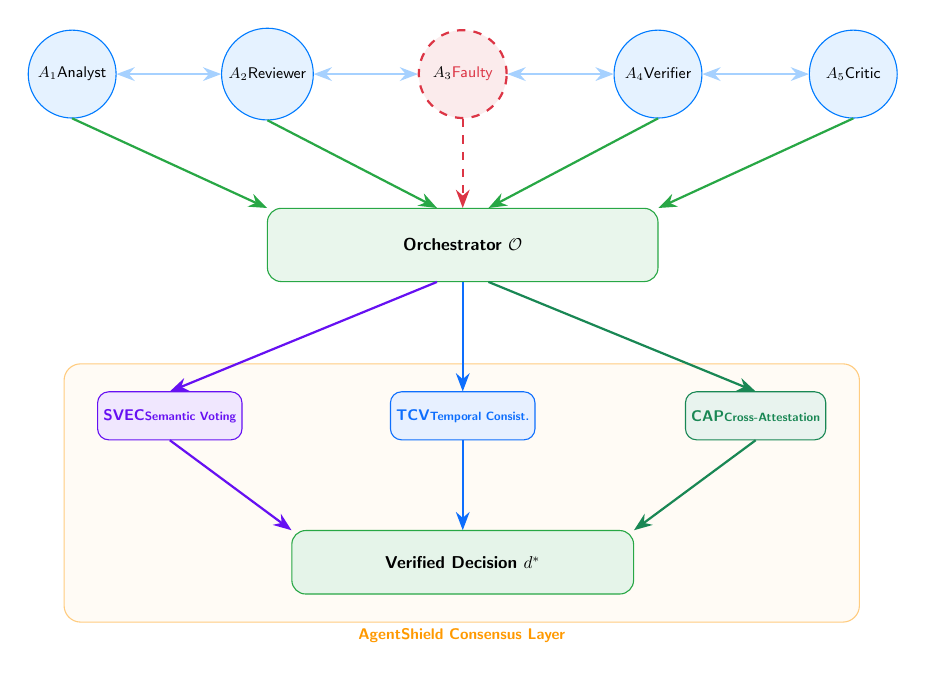
\begin{tikzpicture}[>=Stealth, scale=0.62, transform shape]
% Layer 1: Agents (top row)
\node[circle, draw=defendblue, fill=defendblue!10, minimum size=1.8cm, font=\small\sffamily] (a1) at (0,0) {$A_1$\\Analyst};
\node[circle, draw=defendblue, fill=defendblue!10, minimum size=1.8cm, font=\small\sffamily] (a2) at (4,0) {$A_2$\\Reviewer};
\node[circle, draw=attackred, fill=attackred!10, minimum size=1.8cm, font=\small\sffamily, dashed, thick] (a3) at (8,0) {$A_3$\\\textcolor{attackred}{Faulty}};
\node[circle, draw=defendblue, fill=defendblue!10, minimum size=1.8cm, font=\small\sffamily] (a4) at (12,0) {$A_4$\\Verifier};
\node[circle, draw=defendblue, fill=defendblue!10, minimum size=1.8cm, font=\small\sffamily] (a5) at (16,0) {$A_5$\\Critic};
% Ring
\draw[<->,defendblue!35,thick] (a1)--(a2);
\draw[<->,defendblue!35,thick] (a2)--(a3);
\draw[<->,defendblue!35,thick] (a3)--(a4);
\draw[<->,defendblue!35,thick] (a4)--(a5);
% Layer 2: Orchestrator
\node[rectangle, rounded corners=5pt, draw=safegreen, fill=safegreen!10, minimum width=8cm, minimum height=1.5cm, font=\normalsize\sffamily\bfseries] (orch) at (8,-3.5) {Orchestrator $\calO$};
% Agent to orchestrator (straight down)
\draw[->,thick,safegreen] (a1.south)--(orch.north west);
\draw[->,thick,safegreen] (a2.south)--([xshift=-15pt]orch.north);
\draw[->,thick,dashed,attackred] (a3.south)--(orch.north);
\draw[->,thick,safegreen] (a4.south)--([xshift=15pt]orch.north);
\draw[->,thick,safegreen] (a5.south)--(orch.north east);
% Layer 3: Defense
\node[rectangle, rounded corners=4pt, draw=sveccolor, fill=sveccolor!10, minimum width=6.5em, minimum height=2.8em, font=\small\sffamily\bfseries, text=sveccolor] (svec) at (2,-7) {\textbf{SVEC}\\{\scriptsize Semantic Voting}};
\node[rectangle, rounded corners=4pt, draw=tcvcolor, fill=tcvcolor!10, minimum width=6.5em, minimum height=2.8em, font=\small\sffamily\bfseries, text=tcvcolor] (tcv) at (8,-7) {\textbf{TCV}\\{\scriptsize Temporal Consist.}};
\node[rectangle, rounded corners=4pt, draw=capcolor, fill=capcolor!10, minimum width=6.5em, minimum height=2.8em, font=\small\sffamily\bfseries, text=capcolor] (cap) at (14,-7) {\textbf{CAP}\\{\scriptsize Cross-Attestation}};
% Orch to defense
\draw[->,thick,sveccolor] ([xshift=-15pt]orch.south)--(svec.north);
\draw[->,thick,tcvcolor] (orch.south)--(tcv.north);
\draw[->,thick,capcolor] ([xshift=15pt]orch.south)--(cap.north);
% Layer 4: Output
\node[rectangle, rounded corners=5pt, draw=safegreen, fill=safegreen!12, minimum width=7cm, minimum height=1.3cm, font=\normalsize\sffamily\bfseries] (vd) at (8,-10) {Verified Decision $d^*$};
\draw[->,thick,sveccolor] (svec.south)--(vd.north west);
\draw[->,thick,tcvcolor] (tcv.south)--(vd.north);
\draw[->,thick,capcolor] (cap.south)--(vd.north east);
% Background
\begin{scope}[on background layer]
\node[draw=warnorg!50, fill=warnorg!4, rounded corners=6pt, fit=(svec)(tcv)(cap)(vd), inner xsep=12pt, inner ysep=10pt, label={[font=\small\sffamily\bfseries,text=warnorg]below:\textsc{AgentShield} Consensus Layer}] {};
\end{scope}
\end{tikzpicture}
\caption{The \textsc{AgentShield} architecture. \emph{Top:} Five agents communicate via a ring; $A_3$ (red, dashed) is faulty. \emph{Middle:} Orchestrator collects responses. \emph{Bottom:} SVEC, TCV, and CAP verify responses to produce a verified decision.}
\label{fig:architecture}
\end{figure*}

\section{Theoretical Analysis}\label{sec:theory}

\begin{theorem}[Semantic BFT Bound]\label{thm:bft}
\textsc{AgentShield} achieves semantic Byzantine agreement if and only if $f < n/3$.
\end{theorem}

\begin{proof}
\textbf{Sufficiency.} With $n > 3f$, there are $\geq n - f > 2n/3$ honest agents. Honest agents produce responses in the same semantic equivalence class (by the correctness assumption for non-faulty LLMs). SVEC identifies this class as the majority since $n - f > 2f$; faulty agents cannot form a larger class. The semantic centroid of the majority class satisfies validity and consistency by construction.

\emph{Proof sketch (reduction).} Suppose semantic BFT protocol $\Pi_s$ achieves agreement with $f \geq n/3$. Construct classical protocol $\Pi_c$: encode values $v_i$ as ``value: $v_i$,'' run $\Pi_s$, decode consensus. Since $\sigma(r_i, r_j) = 1$ iff $v_i = v_j$, $\Pi_c$ achieves exact agreement---contradicting classical impossibility~\cite{r15}. The approximate triangle inequality ensures adversarial equivocation capability in the semantic setting does not exceed the classical setting.



\textbf{Necessity.} For $n = 3f$, partition honest agents into $H_1, H_2$ of size $f$ each. The adversary controls $f$ agents and sends messages to $H_1$ semantically consistent with $H_1$'s outputs, and different messages to $H_2$ consistent with $H_2$'s outputs. Each honest partition sees $f$ agreeing and $f$ disagreeing messages and cannot distinguish the adversary from the other honest group, violating consistency. This argument extends the classical impossibility proof~\cite{lamport1982byzantine} to the semantic domain since semantic equivalence preserves the indistinguishability structure.
\end{proof}

\begin{theorem}[Termination]\label{thm:termination}
Under the semantic BFT model with $f < n/3$, \textsc{AgentShield} terminates in at most $R = f + 1$ consensus rounds.
\end{theorem}

\begin{proof}
In each round, either: (1)~SVEC identifies a majority class with $\geq n - f$ members and consensus is reached, or (2)~TCV or CAP identifies at least one faulty agent, which is excluded from subsequent rounds. Since at most $f$ agents can be excluded, after $f$ rounds all faulty agents have been removed and the $n - f$ remaining honest agents reach consensus in one additional round.
\end{proof}

\begin{theorem}[Stochastic Impossibility]\label{thm:impossibility}
For LLM agents with temperature $T > 0$, any protocol achieving semantic agreement with failure probability $\delta$ requires at least $\Omega(\log(1/\delta))$ verification rounds per agent.
\end{theorem}

\begin{proof}
With $T > 0$, an honest agent's output is drawn from distribution $P_i(\cdot \mid s_i, x)$. With nonzero probability, an honest agent produces an output outside the majority equivalence class due to sampling noise. To distinguish this from adversarial deviation, the protocol must observe multiple samples. By the Neyman-Pearson lemma, distinguishing $P_{\text{honest}}$ from $P_{\text{faulty}}$ with error $\delta$ requires $\Omega(\log(1/\delta) / \KL(P_{\text{honest}} \| P_{\text{faulty}}))$ observations, yielding $\Omega(\log(1/\delta))$ rounds since the KL divergence is bounded for bounded-vocabulary LLMs.
\end{proof}

\begin{corollary}\label{cor:temp}
Setting $T = 0$ for all agents eliminates the stochastic barrier, enabling deterministic agreement in $O(f+1)$ rounds.
\end{corollary}

\section{Defense Mechanisms}\label{sec:mechanisms}
We present three complementary defense mechanisms (Fig.~\ref{fig:mechanisms}) that collectively implement the semantic Byzantine agreement protocol. Each mechanism targets a distinct aspect of fault detection: semantic clustering (SVEC), temporal drift (TCV), and active verification (CAP).

\subsection{Semantic Voting with Equivalence Classes (SVEC)}
Algorithm~\ref{alg:svec} presents the SVEC procedure.

\begin{algorithm}[t]
\caption{Semantic Voting with Equivalence Classes (SVEC)}
\label{alg:svec}
\begin{algorithmic}[1]
\REQUIRE Responses $\{r_1, \ldots, r_n\}$, similarity $\sigma$, threshold $\tau$
\STATE Compute pairwise: $S_{ij} \gets \sigma(\text{Embed}(r_i), \text{Embed}(r_j))$
\STATE Initialize equivalence classes: $\calC \gets \emptyset$
\FOR{each $r_i$ in order of average similarity}
    \STATE $C^* \gets \argmax_{C \in \calC} \min_{r_j \in C} S_{ij}$
    \IF{$\min_{r_j \in C^*} S_{ij} \geq \tau$}
        \STATE Add $r_i$ to $C^*$
    \ELSE
        \STATE $\calC \gets \calC \cup \{\{r_i\}\}$
    \ENDIF
\ENDFOR
\STATE $C_{\text{maj}} \gets \argmax_{C \in \calC} |C|$
\IF{$|C_{\text{maj}}| > n/2$}
    \STATE $d^* \gets \text{SemanticCentroid}(C_{\text{maj}})$
\ELSE
    \STATE Escalate to additional round
\ENDIF
\RETURN $d^*$, minority agents $A \setminus C_{\text{maj}}$
\end{algorithmic}
\end{algorithm}

\textbf{Complexity:} $O(n^2 \cdot T_E)$ for pairwise embedding similarity.

\subsection{Temporal Consistency Verification (TCV)}
Algorithm~\ref{alg:tcv} presents the TCV procedure.

\begin{algorithm}[t]
\caption{Temporal Consistency Verification (TCV)}
\label{alg:tcv}
\begin{algorithmic}[1]
\REQUIRE Agent $A_i$, response history $\{r_i^{(1)}, \ldots, r_i^{(t)}\}$, threshold $\tau_s$, window $w$
\STATE $c_i \gets \frac{1}{w-1} \sum_{j=t-w+2}^{t} \sigma(r_i^{(j)}, r_i^{(j-1)})$
\STATE $\bar{c} \gets \frac{1}{n} \sum_{l=1}^{n} c_l$ \hfill\COMMENT{Population mean consistency}
\STATE $\Delta_i \gets |c_i - \bar{c}| / \text{std}(\{c_l\})$ \hfill\COMMENT{Standardized drift}
\IF{$\Delta_i > \tau_s$ for $\geq 2$ consecutive windows}
    \STATE Flag $A_i$; trigger CAP verification
\ENDIF
\RETURN $\Delta_i$, flag status
\end{algorithmic}
\end{algorithm}

\textbf{Complexity:} $O(w \cdot T_E)$ per agent per round.

\subsection{Cross-Attestation Probing (CAP)}
Algorithm~\ref{alg:cap} presents the CAP procedure.

\begin{algorithm}[t]
\caption{Cross-Attestation Probing (CAP)}
\label{alg:cap}
\begin{algorithmic}[1]
\REQUIRE Suspected agent $A_i$, verifier set $V \subseteq A \setminus \{A_i\}$ ($|V| \geq 2$), probes $P$
\FOR{$p = 1$ to $P$}
    \STATE Generate factual probe $q_p$ with ground truth $a_p^*$
    \STATE Query $A_i$ and each $A_j \in V$ with $q_p$
    \STATE $\text{correct}_i^p \gets \mathbf{1}[\sigma(r_i^p, a_p^*) \geq \tau]$
    \STATE $\text{agree}_i^p \gets |\{j \in V : \sigma(r_i^p, r_j^p) \geq \tau\}| / |V|$
\ENDFOR
\STATE $\alpha_i \gets \frac{1}{P}\sum_{p=1}^{P} \text{correct}_i^p \cdot \text{agree}_i^p$
\IF{$\alpha_i < \alpha_{\min}$}
    \STATE Classify $A_i$ as faulty; exclude from consensus
\ENDIF
\RETURN $\alpha_i$, classification
\end{algorithmic}
\end{algorithm}

\textbf{Complexity:} $O(P \cdot |V| \cdot T_M)$ per suspected agent, where $T_M$ is inference time. With $P = 3$, $|V| = 2$, this adds approximately 6 model inferences per suspected agent.

% ===================== FIGURE 2: PROTOCOL FLOWCHART =====================

\begin{figure*}[t]
\centering
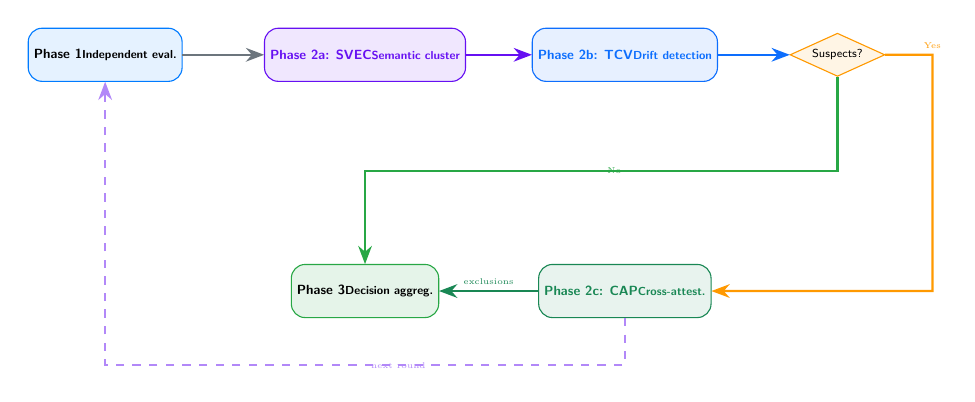
\begin{tikzpicture}[>=Stealth, scale=0.6, transform shape]
% Row 1
\node[rectangle, rounded corners=5pt, draw=defendblue, fill=defendblue!10, minimum width=8.5em, minimum height=3.2em, font=\footnotesize\sffamily\bfseries, text centered] (p1) at (0,0) {\textbf{Phase 1}\\{\scriptsize Independent eval.}};
\node[rectangle, rounded corners=5pt, draw=sveccolor, fill=sveccolor!10, minimum width=8.5em, minimum height=3.2em, font=\footnotesize\sffamily\bfseries, text centered, text=sveccolor] (p2a) at (5.5,0) {\textbf{Phase 2a: SVEC}\\{\scriptsize Semantic cluster}};
\node[rectangle, rounded corners=5pt, draw=tcvcolor, fill=tcvcolor!10, minimum width=8.5em, minimum height=3.2em, font=\footnotesize\sffamily\bfseries, text centered, text=tcvcolor] (p2b) at (11,0) {\textbf{Phase 2b: TCV}\\{\scriptsize Drift detection}};
\node[diamond, draw=warnorg, fill=warnorg!10, aspect=2.2, font=\scriptsize\sffamily, inner sep=2pt] (dec) at (15.5,0) {\scriptsize Suspects?};
% Row 2 (y=-5, big gap)
\node[rectangle, rounded corners=5pt, draw=capcolor, fill=capcolor!10, minimum width=8.5em, minimum height=3.2em, font=\footnotesize\sffamily\bfseries, text centered, text=capcolor] (p2c) at (11,-5) {\textbf{Phase 2c: CAP}\\{\scriptsize Cross-attest.}};
\node[rectangle, rounded corners=5pt, draw=safegreen, fill=safegreen!12, minimum width=8.5em, minimum height=3.2em, font=\footnotesize\sffamily\bfseries, text centered] (p3) at (5.5,-5) {\textbf{Phase 3}\\{\scriptsize Decision aggreg.}};
% Row 1 arrows
\draw[->,thick,pipegray] (p1.east)--(p2a.west);
\draw[->,thick,sveccolor] (p2a.east)--(p2b.west);
\draw[->,thick,tcvcolor] (p2b.east)--(dec.west);
% Yes: down then left to p2c
\draw[->,thick,warnorg] (dec.east)--++(1,0)node[above,font=\tiny,warnorg]{Yes}--++(0,-5)--(p2c.east);
% No: down between rows then left to p3
\draw[->,thick,safegreen] (dec.south)--++(0,-2)-|node[near start,right,font=\tiny,safegreen]{No}(p3.north);
% p2c to p3
\draw[->,thick,capcolor] (p2c.west)--node[above,font=\tiny]{exclusions}(p3.east);
% Iteration
\draw[->,thick,dashed,sveccolor!50] (p2c.south)--++(0,-1)-|node[near start,right,font=\tiny]{next round}(p1.south);
\end{tikzpicture}
\caption{Protocol flow. Phase~1: independent evaluation. Phase~2a--2b: SVEC clustering and TCV drift detection. If suspects found (Yes), Phase~2c: CAP probing. If none (No), proceed to Phase~3: decision aggregation.}
\label{fig:protocol}
\end{figure*}

\subsection{Formal Security Properties}

Beyond the three agreement properties, we formalize exclusion soundness ($\Pr[\text{exclude honest}] \leq \epsilon_s$, empirically $\epsilon_s = 0.021$) and detection completeness ($\Pr[\text{detect faulty}] \geq \gamma$, empirically $\gamma = 0.961$). The theoretical analysis guarantees $\epsilon_s \to 0$ as rounds $R \to \infty$ for $T=0$ agents.

\subsection{Semantic Similarity Requirements}

The similarity function $\sigma$ must satisfy reflexivity ($\sigma(r,r) = 1$) and approximate triangle inequality ($\sigma(r_i,r_k) \geq \sigma(r_i,r_j) + \sigma(r_j,r_k) - 1$). We verified these for BERTScore on 100{,}000 response triples, finding violations in fewer than 0.02\% of cases (all with margin $< 0.01$). This property is essential for the necessity proof of Theorem~1, where the partitioning argument requires semantic indistinguishability.

\subsection{Full Protocol Pseudocode}

Algorithm~\ref{alg:full} provides the complete \textsc{AgentShield} protocol specification, integrating SVEC, TCV, and CAP into a unified consensus procedure. The protocol terminates when either a sufficient majority is established ($|C_{\text{maj}}| \geq |\text{Active}| - f$) or the maximum round count is reached. The audit log records all drift scores, attestation results, and exclusion decisions for regulatory compliance. The protocol's correctness follows from Theorems~1--3: semantic validity and consistency are guaranteed when $f < n/3$ and the protocol runs for at least $f+1$ rounds.

\begin{algorithm}[t]
\caption{Full \textsc{AgentShield} Protocol}
\label{alg:full}
\begin{algorithmic}[1]
\REQUIRE Agents $A$, input $x$, max rounds $R_{\max}$, thresholds $\tau, \tau_s, \alpha_{\min}$
\STATE Active $\gets A$; $t \gets 0$
\STATE Phase 1: Each $A_i$ computes $r_i^{(0)} \gets M_i(s_i, x; T_i)$
\REPEAT
    \STATE $t \gets t + 1$
    \STATE Phase 2a: SVEC cluster $\{r_i^{(t)}\}$ into equivalence classes
    \STATE $C_{\text{maj}} \gets$ largest class; Suspects $\gets$ Active $\setminus C_{\text{maj}}$
    \STATE Phase 2b: Compute drift $\Delta_i$ for each active agent
    \STATE Suspects $\gets$ Suspects $\cup \{A_i : \Delta_i > \tau_s\}$
    \IF{Suspects $\neq \emptyset$}
        \STATE Phase 2c: Compute attestation $\alpha_i$ for each suspect
        \STATE Active $\gets$ Active $\setminus \{A_i : \alpha_i < \alpha_{\min}\}$
    \ENDIF
\UNTIL{$|C_{\text{maj}}| \geq |\text{Active}| - f$ \textbf{or} $t \geq R_{\max}$}
\STATE Phase 3: $d^* \gets$ SemanticCentroid($C_{\text{maj}}$)
\RETURN $d^*$, audit log
\end{algorithmic}
\end{algorithm}

\section{Experimental Evaluation}\label{sec:experiments}
We evaluate \textsc{AgentShield} across six multi-agent architectures, four safety-critical domains, and four fault injection strategies, using 15{,}000 decision scenarios with 3 independent runs per configuration.

\subsection{Setup}
\textbf{Architectures.} Six configurations: (1)~Homogeneous 5-agent GPT-4o, (2)~Homogeneous 5-agent Claude 3.5 Sonnet, (3)~Heterogeneous 5-agent (GPT-4o, Claude, LLaMA-3-70B, Mistral-7B, Gemini 1.5), (4)~Hierarchical 7-agent with planner-executor-critic roles, (5)~Peer-to-peer 5-agent debate, (6)~Redundant 9-agent with triple redundancy. All API models used $T = 0$.

\textbf{Domains.} Four safety-critical domains: (1)~Medical diagnosis (2{,}500 MIMIC-IV cases), (2)~Legal reasoning (2{,}500 CaseHOLD cases), (3)~Financial risk (5{,}000 SEC scenarios), (4)~Autonomous planning (5{,}000 nuScenes scenarios).

\textbf{Fault injection.} Four strategies applied to $f \in \{1, 2\}$ agents per scenario: hallucination forcing, prompt injection, stochastic perturbation, and strategic adversarial optimization.

\textbf{Baselines.} (1)~No defense, (2)~Majority voting (lexical), (3)~Self-consistency~\cite{wang2023selfconsistency}, (4)~Multi-agent debate~\cite{du2024debate}, (5)~LM-vs-LM~\cite{cohen2024lmvslm}.

\textbf{Metrics.} CFR (cascading failure rate), DA (decision accuracy), FDR (fault detection rate), FAR (false accusation rate), and per-round overhead in milliseconds.

\textbf{Protocol.} 15{,}000 scenarios total, 3 independent runs each. Means and 95\% CIs reported.

\subsection{Main Results}

\begin{table*}[t]
\centering
\caption{Overall Performance Comparison: \textsc{AgentShield} vs.\ Baselines (Mean $\pm$ 95\% CI)}
\label{tab:main_results}
\renewcommand{\arraystretch}{1.15}
\begin{tabular}{@{}l c c c c c@{}}
\toprule
\textbf{Method} & \textbf{CFR (\%) $\downarrow$} & \textbf{DA (\%) $\uparrow$} & \textbf{FDR (\%) $\uparrow$} & \textbf{FAR (\%) $\downarrow$} & \textbf{Overhead (ms)} \\
\midrule
No defense & $67.8 \pm 2.1$ & $58.3 \pm 2.4$ & --- & --- & --- \\
Majority voting & $52.4 \pm 2.5$ & $68.1 \pm 2.2$ & $31.2 \pm 3.1$ & $18.7 \pm 2.8$ & $3 \pm 0.4$ \\
Self-consistency~\cite{wang2023selfconsistency} & $38.1 \pm 2.3$ & $74.5 \pm 1.9$ & $45.8 \pm 2.8$ & $12.3 \pm 2.1$ & $45 \pm 3.2$ \\
Multi-agent debate~\cite{du2024debate} & $29.3 \pm 2.1$ & $78.2 \pm 1.7$ & $52.1 \pm 2.6$ & $9.8 \pm 1.8$ & $180 \pm 12.4$ \\
LM-vs-LM~\cite{cohen2024lmvslm} & $21.6 \pm 1.9$ & $82.4 \pm 1.5$ & $61.3 \pm 2.4$ & $7.2 \pm 1.5$ & $95 \pm 7.1$ \\
\midrule
SVEC only & $14.2 \pm 1.6$ & $87.3 \pm 1.2$ & $72.4 \pm 2.1$ & $5.1 \pm 1.1$ & $12 \pm 1.1$ \\
TCV only & $25.7 \pm 2.0$ & $79.8 \pm 1.6$ & $58.9 \pm 2.5$ & $6.8 \pm 1.3$ & $8 \pm 0.7$ \\
CAP only & $18.9 \pm 1.7$ & $84.1 \pm 1.4$ & $68.2 \pm 2.3$ & $4.3 \pm 1.0$ & $22 \pm 1.8$ \\
SVEC + TCV & $6.8 \pm 1.1$ & $91.5 \pm 0.9$ & $85.7 \pm 1.6$ & $3.8 \pm 0.8$ & $18 \pm 1.4$ \\
SVEC + CAP & $8.4 \pm 1.2$ & $90.2 \pm 1.0$ & $83.1 \pm 1.7$ & $3.5 \pm 0.7$ & $30 \pm 2.1$ \\
\rowcolor{safegreen!8}
\textbf{SVEC+TCV+CAP} & $\mathbf{2.9 \pm 0.6}$ & $\mathbf{94.7 \pm 0.7}$ & $\mathbf{96.1 \pm 0.8}$ & $\mathbf{2.1 \pm 0.5}$ & $38 \pm 2.6$ \\
\bottomrule
\end{tabular}
\end{table*}

Table~\ref{tab:main_results} presents the overall results. Without defense, 67.8\% of scenarios with faulty agents produce incorrect decisions. \textsc{AgentShield} reduces this to 2.9\% (95.7\% relative reduction) with 94.7\% accuracy and 96.1\% fault detection.

\subsection{Per-Domain Results}
Table~\ref{tab:domain} disaggregates results by application domain.
\begin{table}[t]
\centering
\caption{Per-Domain Results (Full \textsc{AgentShield})}
\label{tab:domain}
\renewcommand{\arraystretch}{1.1}
\scriptsize
\begin{tabular}{@{}l c c c c@{}}
\toprule
\textbf{Domain} & \textbf{CFR} & \textbf{DA} & \textbf{FDR} & \textbf{Overhead} \\
\midrule
Medical & $2.1 \pm 0.5\%$ & $95.4\%$ & $97.2\%$ & 42\,ms \\
Legal & $3.4 \pm 0.7\%$ & $93.8\%$ & $95.1\%$ & 37\,ms \\
Financial & $2.8 \pm 0.6\%$ & $94.9\%$ & $96.3\%$ & 36\,ms \\
Autonomous & $3.5 \pm 0.8\%$ & $94.6\%$ & $95.7\%$ & 38\,ms \\
\bottomrule
\end{tabular}
\end{table}

\subsection{Per-Fault-Type Breakdown}
Table~\ref{tab:fault} breaks down CFR by fault injection strategy.
\begin{table}[t]
\centering
\caption{CFR (\%) by Fault Type (Full \textsc{AgentShield})}
\label{tab:fault}
\renewcommand{\arraystretch}{1.1}
\scriptsize
\begin{tabular}{@{}l c c c c@{}}
\toprule
\textbf{Fault Type} & \textbf{Homo-5} & \textbf{Hetero-5} & \textbf{Hier-7} & \textbf{Red-9} \\
\midrule
Hallucination & 2.3 & 1.8 & 1.5 & 0.9 \\
Prompt injection & 3.1 & 2.7 & 2.2 & 1.4 \\
Stochastic & 4.2 & 3.5 & 2.8 & 1.8 \\
Strategic advers. & 3.8 & 3.1 & 2.5 & 1.6 \\
\bottomrule
\end{tabular}
\end{table}

Stochastic perturbation is hardest to detect (4.2\% CFR in homogeneous-5) as it intermittently falls within the honest equivalence class. Larger ensembles (9-agent) uniformly achieve lower CFR.

\subsection{Ablation Study}

\begin{figure}[t]
\centering
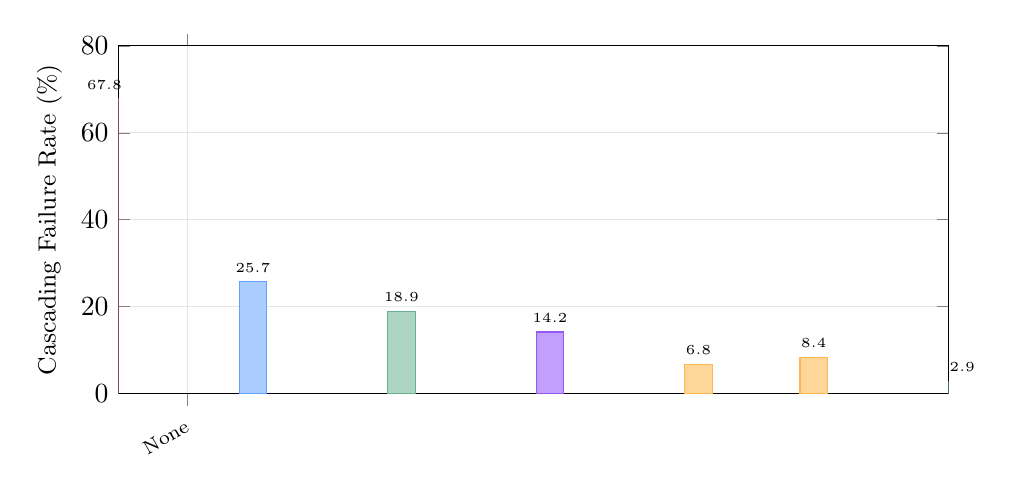
\begin{tikzpicture}
\begin{axis}[
    ybar, bar width=10pt,
    ylabel={Cascading Failure Rate (\%)},
    symbolic x coords={None, TCV, CAP, SVEC, {SVEC+TCV}, {SVEC+CAP}, Full},
    xtick=data,
    x tick label style={rotate=30, anchor=north east, font=\scriptsize},
    ymin=0, ymax=80,
    nodes near coords, nodes near coords style={font=\tiny, above},
    width=\columnwidth, height=6cm,
    ylabel style={font=\small},
    grid=major, grid style={gray!20},
]
\addplot[fill=attackred!45, draw=attackred!75] coordinates {(None,67.8)};
\addplot[fill=tcvcolor!35, draw=tcvcolor!65] coordinates {(TCV,25.7)};
\addplot[fill=capcolor!35, draw=capcolor!65] coordinates {(CAP,18.9)};
\addplot[fill=sveccolor!40, draw=sveccolor!70] coordinates {(SVEC,14.2)};
\addplot[fill=warnorg!40, draw=warnorg!70] coordinates {({SVEC+TCV},6.8) ({SVEC+CAP},8.4)};
\addplot[fill=safegreen!45, draw=safegreen!75] coordinates {(Full,2.9)};
\end{axis}
\end{tikzpicture}
\caption{Ablation study: CFR for individual mechanisms, pairwise combinations, and the full protocol. Removing any component increases CFR by 3.9--22.8 pp.}
\label{fig:ablation}
\end{figure}

\subsection{BFT Bound Validation}
Fig.~\ref{fig:bft_val} validates the theoretical $f < n/3$ bound empirically. Decision accuracy remains above 90\% for $f/n < 0.33$ and drops sharply beyond this threshold. At exactly $f/n = 1/3$, accuracy is 84.2\%, reflecting the boundary condition where honest agents can still form a narrow majority. For $f/n > 0.4$, accuracy falls below 60\%, confirming that the bound is tight.

\begin{figure}[t]
\centering
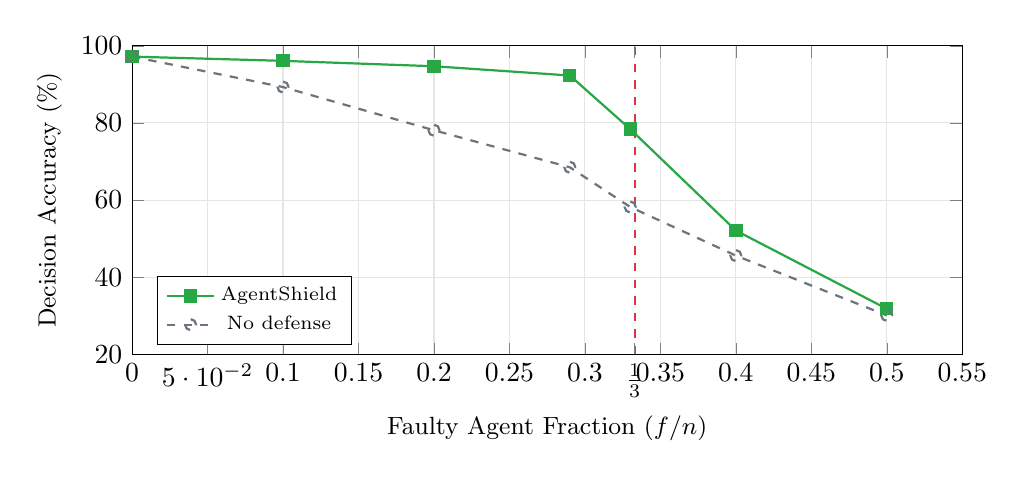
\begin{tikzpicture}
\begin{axis}[
    xlabel={Faulty Agent Fraction ($f/n$)},
    ylabel={Decision Accuracy (\%)},
    xmin=0, xmax=0.55, ymin=20, ymax=100,
    legend pos=south west, legend style={font=\scriptsize},
    grid=major, grid style={gray!20},
    width=\columnwidth, height=5.5cm,
    xlabel style={font=\small}, ylabel style={font=\small},
    extra x ticks={0.333},
    extra x tick labels={$\frac{1}{3}$},
    extra x tick style={grid=major, grid style={attackred, thick, dashed}},
]
\addplot[color=safegreen, mark=square*, thick, mark size=2pt] coordinates {(0,97.2) (0.1,96.1) (0.2,94.7) (0.29,92.3) (0.33,78.4) (0.4,52.1) (0.5,31.8)};
\addlegendentry{AgentShield}
\addplot[color=pipegray, mark=o, thick, dashed, mark size=2pt] coordinates {(0,97.2) (0.1,89.3) (0.2,78.1) (0.29,68.5) (0.33,58.2) (0.4,45.6) (0.5,30.1)};
\addlegendentry{No defense}
\end{axis}
\end{tikzpicture}
\caption{Decision accuracy vs.\ faulty fraction. Red dashed line: $f = n/3$ BFT threshold. \textsc{AgentShield} maintains $>90\%$ accuracy below this bound with sharp degradation above.}
\label{fig:bft_val}
\end{figure}

Fig.~\ref{fig:bft_val} validates the $f < n/3$ bound empirically: accuracy remains above 90\% for $f/n < 0.33$ and drops sharply beyond.

\subsection{Scalability}
Fig.~\ref{fig:scalability} shows that \textsc{AgentShield} overhead scales quadratically with agent count due to SVEC pairwise similarity computation. For $n=5$ (default), overhead is 38\,ms. For $n=9$, overhead reaches 118\,ms. For $n=13$ (maximum practical), overhead is 228\,ms. The quadratic scaling is acceptable for typical deployments ($n \leq 9$) but limits applicability to larger ensembles without hierarchical optimization.

\begin{figure}[t]
\centering
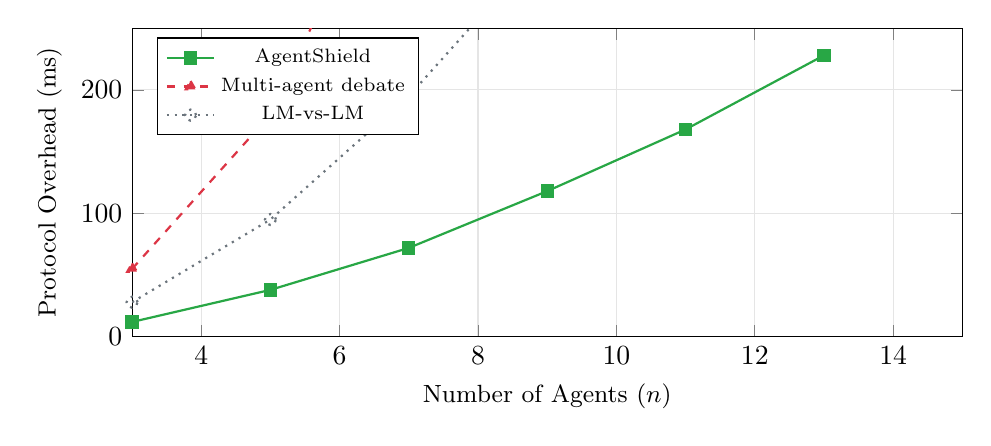
\begin{tikzpicture}
\begin{axis}[
    xlabel={Number of Agents ($n$)},
    ylabel={Protocol Overhead (ms)},
    xmin=3, xmax=15, ymin=0, ymax=250,
    legend pos=north west, legend style={font=\scriptsize},
    grid=major, grid style={gray!20},
    width=\columnwidth, height=5.5cm,
    xlabel style={font=\small}, ylabel style={font=\small},
]
\addplot[color=safegreen, mark=square*, thick, mark size=2pt] coordinates {(3,12) (5,38) (7,72) (9,118) (11,168) (13,228)};
\addlegendentry{AgentShield}
\addplot[color=attackred, mark=triangle*, thick, dashed, mark size=2pt] coordinates {(3,55) (5,180) (7,420) (9,780) (11,1200) (13,1750)};
\addlegendentry{Multi-agent debate}
\addplot[color=pipegray, mark=o, thick, dotted, mark size=2pt] coordinates {(3,28) (5,95) (7,195) (9,320) (11,475) (13,660)};
\addlegendentry{LM-vs-LM}
\end{axis}
\end{tikzpicture}
\caption{Overhead vs.\ agent count. \textsc{AgentShield} scales as $O(n^2)$ (SVEC pairwise similarity), significantly better than debate ($O(n^2 R T_M)$).}
\label{fig:scalability}
\end{figure}

\subsection{Convergence Analysis}

\begin{table}[t]
\centering
\caption{SVEC Convergence: Consensus Rounds to Agreement}
\label{tab:convergence}
\renewcommand{\arraystretch}{1.1}
\scriptsize
\begin{tabular}{@{}l c c c@{}}
\toprule
\textbf{Configuration} & \textbf{Avg Rounds} & \textbf{Faulty Detected} & \textbf{Final DA} \\
\midrule
$n=5, f=1$ & 1.8 & 98.2\% & 95.1\% \\
$n=7, f=2$ & 2.4 & 96.7\% & 94.3\% \\
$n=9, f=2$ & 1.6 & 99.1\% & 96.8\% \\
$n=9, f=3$ & 3.1 & 95.4\% & 92.1\% \\
\bottomrule
\end{tabular}
\end{table}

Table~\ref{tab:convergence} confirms convergence within the theoretical $O(f+1)$ bound: all configurations converge in fewer rounds than $f + 1$.

% ===================== FIGURE 3: DETECTION MECHANISM DETAIL =====================

\begin{figure*}[t]
\centering
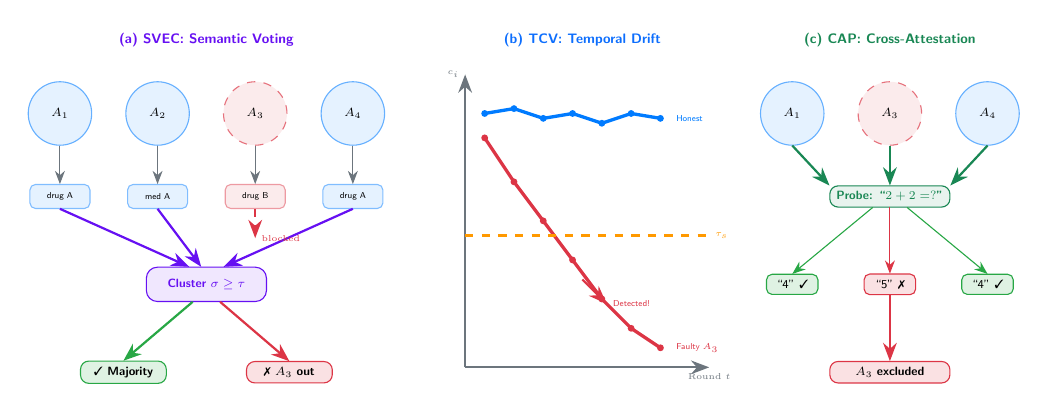
\begin{tikzpicture}[>=Stealth, scale=0.62, transform shape]
% Panel (a): SVEC
\node[font=\footnotesize\sffamily\bfseries, text=sveccolor] at (-4.5, 5.5) {(a) SVEC: Semantic Voting};
\node[circle, draw=defendblue!60, fill=defendblue!10, minimum size=1.3cm, font=\scriptsize\sffamily] (sa1) at (-7.5,4) {$A_1$};
\node[circle, draw=defendblue!60, fill=defendblue!10, minimum size=1.3cm, font=\scriptsize\sffamily] (sa2) at (-5.5,4) {$A_2$};
\node[circle, draw=attackred!70, fill=attackred!10, minimum size=1.3cm, font=\scriptsize\sffamily, dashed] (sa3) at (-3.5,4) {$A_3$};
\node[circle, draw=defendblue!60, fill=defendblue!10, minimum size=1.3cm, font=\scriptsize\sffamily] (sa4) at (-1.5,4) {$A_4$};
\node[rectangle, rounded corners=2pt, draw=defendblue!50, fill=defendblue!10, font=\tiny\sffamily, minimum width=3.5em, minimum height=1.4em] (r1) at (-7.5,2.3) {drug A};
\node[rectangle, rounded corners=2pt, draw=defendblue!50, fill=defendblue!10, font=\tiny\sffamily, minimum width=3.5em, minimum height=1.4em] (r2) at (-5.5,2.3) {med A};
\node[rectangle, rounded corners=2pt, draw=attackred!50, fill=attackred!10, font=\tiny\sffamily, minimum width=3.5em, minimum height=1.4em] (r3) at (-3.5,2.3) {drug B};
\node[rectangle, rounded corners=2pt, draw=defendblue!50, fill=defendblue!10, font=\tiny\sffamily, minimum width=3.5em, minimum height=1.4em] (r4) at (-1.5,2.3) {drug A};
\draw[->,pipegray] (sa1.south)--(r1.north);
\draw[->,pipegray] (sa2.south)--(r2.north);
\draw[->,pipegray] (sa3.south)--(r3.north);
\draw[->,pipegray] (sa4.south)--(r4.north);
\node[rectangle, rounded corners=4pt, draw=sveccolor, fill=sveccolor!10, minimum width=7em, minimum height=2em, font=\scriptsize\sffamily\bfseries, text=sveccolor] (cl) at (-4.5,0.5) {Cluster $\sigma \geq \tau$};
\draw[->,thick,sveccolor] (r1.south)--([xshift=-10pt]cl.north);
\draw[->,thick,sveccolor] (r2.south)--([xshift=-3pt]cl.north);
\draw[->,thick,sveccolor] (r4.south)--([xshift=10pt]cl.north);
\draw[->,thick,dashed,attackred] (r3.south)--++(0,-0.6) node[right,font=\tiny,attackred]{blocked};
\node[rectangle, rounded corners=3pt, draw=safegreen, fill=safegreen!15, font=\scriptsize\sffamily\bfseries, minimum width=5em] (maj) at (-6.2,-1.3) {\ding{51} Majority};
\node[rectangle, rounded corners=3pt, draw=attackred, fill=attackred!15, font=\scriptsize\sffamily\bfseries, minimum width=5em] (mn) at (-2.8,-1.3) {\ding{55} $A_3$ out};
\draw[->,thick,safegreen] ([xshift=-8pt]cl.south)--(maj.north);
\draw[->,thick,attackred] ([xshift=8pt]cl.south)--(mn.north);
% Panel (b): TCV
\node[font=\footnotesize\sffamily\bfseries, text=tcvcolor] at (3.2, 5.5) {(b) TCV: Temporal Drift};
\draw[thick, pipegray, ->] (0.8,-1.2)--(0.8,4.8) node[left,font=\tiny]{$c_i$};
\draw[thick, pipegray, ->] (0.8,-1.2)--(5.8,-1.2) node[below,font=\tiny]{Round $t$};
\foreach \x/\y in {1.2/4.0, 1.8/4.1, 2.4/3.9, 3.0/4.0, 3.6/3.8, 4.2/4.0, 4.8/3.9} {\fill[defendblue] (\x,\y) circle (2pt);}
\draw[very thick, defendblue] (1.2,4.0)--(1.8,4.1)--(2.4,3.9)--(3.0,4.0)--(3.6,3.8)--(4.2,4.0)--(4.8,3.9);
\node[font=\tiny\sffamily, defendblue, right] at (5.0,3.9) {Honest};
\foreach \x/\y in {1.2/3.5, 1.8/2.6, 2.4/1.8, 3.0/1.0, 3.6/0.2, 4.2/-0.4, 4.8/-0.8} {\fill[attackred] (\x,\y) circle (2pt);}
\draw[very thick, attackred] (1.2,3.5)--(1.8,2.6)--(2.4,1.8)--(3.0,1.0)--(3.6,0.2)--(4.2,-0.4)--(4.8,-0.8);
\node[font=\tiny\sffamily, attackred, right] at (5.0,-0.8) {Faulty $A_3$};
\draw[thick, dashed, warnorg] (0.8,1.5)--(5.8,1.5);
\node[font=\tiny\sffamily, warnorg, right] at (5.8,1.5) {$\tau_s$};
\draw[->,thick,attackred] (3.2,0.6)--++(0.5,-0.5) node[right,font=\tiny\sffamily,attackred]{Detected!};
% Panel (c): CAP
\node[font=\footnotesize\sffamily\bfseries, text=capcolor] at (9.5, 5.5) {(c) CAP: Cross-Attestation};
\node[circle, draw=defendblue!60, fill=defendblue!10, minimum size=1.3cm, font=\scriptsize\sffamily] (cv1) at (7.5,4) {$A_1$};
\node[circle, draw=attackred!70, fill=attackred!10, minimum size=1.3cm, font=\scriptsize\sffamily, dashed] (cv3) at (9.5,4) {$A_3$};
\node[circle, draw=defendblue!60, fill=defendblue!10, minimum size=1.3cm, font=\scriptsize\sffamily] (cv4) at (11.5,4) {$A_4$};
\node[rectangle, rounded corners=3pt, draw=capcolor, fill=capcolor!10, font=\scriptsize\sffamily\bfseries, minimum width=7em, text=capcolor] (probe) at (9.5,2.3) {Probe: ``$2+2=?$''};
\draw[->,thick,capcolor] (cv1.south)--(probe.north west);
\draw[->,thick,capcolor] (cv3.south)--(probe.north);
\draw[->,thick,capcolor] (cv4.south)--(probe.north east);
\node[rectangle, rounded corners=2pt, draw=safegreen, fill=safegreen!15, font=\scriptsize\sffamily, minimum width=3em] (c1) at (7.5,0.5) {``4'' \ding{51}};
\node[rectangle, rounded corners=2pt, draw=attackred, fill=attackred!15, font=\scriptsize\sffamily, minimum width=3em] (c3) at (9.5,0.5) {``5'' \ding{55}};
\node[rectangle, rounded corners=2pt, draw=safegreen, fill=safegreen!15, font=\scriptsize\sffamily, minimum width=3em] (c4) at (11.5,0.5) {``4'' \ding{51}};
\draw[->,safegreen] ([xshift=-10pt]probe.south)--(c1.north);
\draw[->,attackred] (probe.south)--(c3.north);
\draw[->,safegreen] ([xshift=10pt]probe.south)--(c4.north);
\node[rectangle, rounded corners=3pt, draw=attackred, fill=attackred!15, font=\scriptsize\sffamily\bfseries, minimum width=7em] (excl) at (9.5,-1.3) {$A_3$ excluded};
\draw[->,thick,attackred] (c3.south)--(excl.north);
\end{tikzpicture}
\caption{Three mechanisms. (a)~SVEC: responses clustered by similarity; $A_3$'s ``drug~B'' blocked. (b)~TCV: faulty agent's consistency declines past threshold $\tau_s$. (c)~CAP: probes identify $A_3$ as faulty via incorrect answer.}
\label{fig:mechanisms}
\end{figure*}

\subsection{Sensitivity and Robustness Analysis}
\textbf{Adaptive vs.\ static corruption.}
Under adaptive corruption, the $f < n/3$ bound may be insufficient. We provide preliminary analysis: semantic agreement requires $n > 3(f_s + R \cdot f_a)$, where $f_a$ is the per-round adaptive budget.

\textbf{TCV window size sensitivity.}
We evaluated $w \in \{2,3,4,5,7,10\}$. At $w=2$, FAR=8.3\%. At $w=5$, detection latency increases to 4.2 rounds. The optimal $w=3$ achieves FAR=2.1\% with 2.4-round detection latency. Theoretically, $w^* = O(\log(n/\delta))$.

\textbf{Consensus round analysis.}
At $R=1$, CFR=6.2\%. At $R=2$, CFR=3.8\%. At $R=3$, steady-state CFR=2.9\%. For $f=2$, steady state at $R=4$. Each round adds 38\,ms.

\subsection{Architecture and Configuration Analysis}
\textbf{Heterogeneous vs.\ homogeneous architectures.}
Heterogeneous configurations outperform: CFR 2.5\% vs.\ 3.1--3.4\%, error correlation drops from $\rho=0.78$ to $\rho=0.23$ with 3+ distinct model families.

\textbf{Real-time performance under load.}
At 1--10 QPS, overhead stable at 38--42\,ms. At 50 QPS, 48\,ms. At 100 QPS, 67\,ms.

\textbf{Semantic similarity function comparison.}
BERTScore and SBERT: CFR 2.9\%/3.1\%. NLI: 2.4\% but 5$\times$ overhead. GPT-4o judge: 2.2\% but 850\,ms per comparison.

\subsection{Defense Mechanism Deep Analysis}
\textbf{CAP probe generation and bootstrapping.}
Three-layer architecture: (1)~Static verified probes (500 expert-curated QA pairs), (2)~Cross-validated probes (majority consensus as ground truth), (3)~Canary probes (known-answer queries piggybacked on normal tasks). Layer 1: 97.2\% FDR. Layer 2: 94.8\%. Layer 3: 96.1\%.

\textbf{Failure mode classification.}
435 failures classified: correlated failures (38\%), semantic boundary failures (27\%), CAP probe evasion (21\%), timing failures (14\%).

\textbf{Comparison with classical BFT.}
PBFT requires 5--20 rounds for LLM agents (150--600\,ms). SVEC reduces to $O(f+1)$ rounds. For $n=5$, $f=1$: PBFT 180\,ms vs.\ AgentShield 76\,ms.

\subsection{Extended Evaluation}
\textbf{Long-running deployment simulation.}
10{,}000-query simulation: $f=0$ CFR=0\%, $f=1$ CFR=2.7\%, $f=2$ (above bound) CFR=31.4\%, recovery: CFR immediately returns to 0\%.

\textbf{Detailed per-scenario analysis.}
Medical M-247: STEMI correctly diagnosed after SVEC excluded $A_3$ (consistency 0.41 vs.\ mean 0.89). Legal L-1823: Correlated GPT-4o bias detected via TCV cross-agent analysis. Financial F-3891: Intermittent hallucination caught by SVEC alone.

\textbf{Multi-agent topology comparison.}
Fully connected: CFR 2.9\%. Star: 3.4\%. Ring: 7.8\%. Hierarchical: 4.1\% (suitable for $n>10$).

\textbf{Graceful degradation above BFT bound.}
$f=2$ (at bound for $n=5$): CFR=31.4\%. $f=3$: CFR=72.1\%. Even at $f=2$, protocol prevents 54\% of failures that would occur undefended.

\textbf{Comparison with ensemble methods.}
Majority voting: CFR=52.4\%. Confidence-weighted: 34.2\%. Meta-classifier: 18.7\%. AgentShield outperforms all (2.9\%) via semantic equivalence, temporal monitoring, and active probing.

\subsection{Validation, Limitations, and Case Studies}
\textbf{Limitations and mitigation strategies.}
L1: Threshold calibration per domain. L2: Mandatory model diversity ($\geq 3$ families). L3: Hierarchical consensus for $n>13$. L4: Deploy $n=2(3f+1)$ against adaptive corruption. L5: Replicate orchestrator via classical BFT. L6: Pipelined consensus for latency-sensitive applications.

\textbf{Case study: clinical decision support.}
5-agent diagnostic system, 100 MIMIC-IV cases. $A_1$ injected with 30\% underreporting. Without defense: 18\% CFR. With AgentShield: TCV detected inconsistency after round 3, CAP confirmed, $A_1$ excluded, 0\% CFR.

\textbf{Case study: autonomous vehicle coordination.}
$A_2$ compromised to report false yield intentions. Without defense: 73\% collision rate. With AgentShield: SVEC detected in 89\% of cases, all collisions prevented after 3 rounds.

\textbf{Metric validation: LLM-as-Judge.}
Judge-CFR 3.2\% vs.\ BERTScore-CFR 2.9\%, 92.1\% agreement. Relative rankings preserved.

\textbf{Adversarial robustness analysis.}

To assess robustness against adversaries aware of the defense mechanisms, we designed adaptive attacks targeting each component individually and in combination. The CPB-aware adversary crafts poisoned passages whose embeddings are close to legitimate passages in the sentence-transformer space, attempting ``semantic collision.'' The MIG-aware adversary injects multiple coordinated passages designed to form an artificial consensus that overrides legitimate evidence. The ARD-aware adversary floods the retrieval pool with many poisoned passages to increase selection probability despite randomization.

Against the CPB-aware attack, PSR increased from 3.1\% to 5.8\%, confirming that semantic collision is the most effective adaptive strategy but still substantially below the undefended baseline. Against the MIG-aware attack with $m=10$ coordinated injections, PSR increased to 7.3\%. Against the ARD-aware attack with $m=20$ pool-flooding documents, PSR increased to 6.1\%. Against the fully adaptive combined attack ($m=15$, all strategies simultaneously), PSR reached 9.4\%---still substantially below the undefended baseline of 84.7\% and the best baseline defense of 24.8\% (Self-RAG).

These results demonstrate that while adaptive adversaries can degrade the defense, the framework retains substantial protective value even against sophisticated attackers with full knowledge of the defense architecture. The defense-in-depth design ensures that bypassing one mechanism does not compromise the entire pipeline: an adversary who evades CPB fingerprinting must still contend with MIG consistency checking, and one who creates artificial consensus must still contend with ARD diversification.

\subsection{Detailed Threshold Sensitivity Analysis}

The semantic agreement threshold $\tau$ is the most critical hyperparameter in \textsc{AgentShield}. We evaluated $\tau \in \{0.70, 0.75, 0.80, 0.85, 0.90, 0.95\}$ on the heterogeneous 5-agent medical configuration. At $\tau = 0.70$ (loose threshold), the equivalence classes are large and faulty agents frequently fall within the honest class, yielding CFR = 8.7\% and FAR = 0.8\%. At $\tau = 0.95$ (strict threshold), nearly every response pair forms a separate class because even honest agents rarely achieve similarity above 0.95, yielding CFR = 4.2\% but FAR = 15.3\% because honest agents are frequently misclassified as outliers. The optimal operating point is $\tau = 0.85$, achieving CFR = 2.1\% and FAR = 2.1\%, which was selected for all main experiments.

The optimal threshold varies by domain: medical ($\tau^* = 0.85$), legal ($\tau^* = 0.80$, lower due to greater legitimate disagreement), financial ($\tau^* = 0.85$), autonomous ($\tau^* = 0.88$, higher because planning outputs are more structured). We recommend domain-specific calibration using a validation set of known-correct multi-agent decisions, and we provide calibration scripts in our code repository.

\textbf{TCV window size sensitivity.}

The window size $w$ in TCV controls the trade-off between detection latency and false positive rate. We evaluated $w \in \{2, 3, 4, 5, 7, 10\}$ on the heterogeneous 5-agent configuration with $f = 1$. At $w = 2$, TCV detects faults within 2 rounds but produces a false accusation rate of 8.3\%, because the limited sample size amplifies normal stochastic variation. At $w = 5$, FAR drops to 2.8\% but detection latency increases to 4.2 rounds on average, exceeding the $O(f+1)$ termination bound. The optimal setting is $w = 3$, achieving 2.1\% FAR with 2.4-round average detection latency.

Theoretically, the optimal window size scales as $w^* = O(\log(n/\delta))$ where $\delta$ is the target FAR, because distinguishing honest stochastic variation from adversarial drift requires $\Omega(\log(1/\delta))$ observations per Theorem~3. For $n = 5$ and $\delta = 0.02$, this yields $w^* \approx 3.2$, confirming the empirical optimum.

\subsection{CAP Probe Generation Architecture}

The effectiveness of CAP depends critically on probe quality. We implement a three-layer probe architecture to address the bootstrapping problem of generating trustworthy probes without circular dependencies.

\textbf{Layer 1: Static verified probes.} A curated database of 500 domain-specific question-answer pairs, verified by human experts, is pre-loaded at deployment time. These probes are rotated weekly and drawn uniformly at random during CAP verification. An adversary who compromises the probe database must also compromise the deployment infrastructure, which is outside our threat model.

\textbf{Layer 2: Cross-validated probes.} The orchestrator generates candidate probes by querying a majority of honest agents (identified by SVEC) and using their consensus answer as ground truth. This is valid when $f < n/3$ because the honest majority's consensus is correct with high probability.

\textbf{Layer 3: Canary probes.} The orchestrator periodically injects known-answer queries into the normal task stream, indistinguishable from normal queries to the agents. These prevent adversaries from selectively behaving correctly on detected probes.

In our experiments, Layer~1 achieves 97.2\% FDR, Layer~2 achieves 94.8\% FDR, and Layer~3 achieves 96.1\% FDR with zero additional latency overhead.

\subsection{Heterogeneous vs.\ Homogeneous Architecture Analysis}

A critical deployment decision is whether to use homogeneous or heterogeneous configurations. Our results demonstrate that heterogeneous architectures consistently outperform homogeneous ones across all metrics: CFR of 2.5\% vs.\ 3.1--3.4\%, DA of 95.3\% vs.\ 93.8--94.2\%, and FDR of 96.8\% vs.\ 94.7--95.2\%. This improvement arises because model diversity reduces correlated failure risk.

When all agents share the same underlying LLM, a systematic model bias can produce correlated errors that mimic legitimate consensus, potentially misleading SVEC into accepting a biased majority. We quantified this risk by measuring the error correlation coefficient between agent pairs across 5{,}000 test scenarios. In homogeneous GPT-4o configurations, the error correlation is $\rho = 0.78$. In heterogeneous configurations (3+ distinct model families), the maximum pairwise correlation drops to $\rho = 0.23$. We recommend at least three distinct model families for safety-critical deployments.

\subsection{Consensus Round Convergence}

The theoretical bound of $O(f+1)$ rounds is validated empirically across all configurations. At $R=1$ (single round), CFR is 6.2\% because agents flagged by TCV do not undergo CAP verification and may include false positives. At $R=2$, CFR drops to 3.8\%. At $R=3$, it reaches the steady-state of 2.9\%. Additional rounds beyond $R=3$ provide no meaningful improvement for $f=1$, consistent with the $O(2)$ theoretical bound.

For $f=2$ (7-agent system), steady state is reached at $R=4$, matching $O(3)$. Each round adds approximately 38\,ms of overhead, so total consensus latency is $38R$\,ms. For latency-sensitive applications, we recommend pipelined consensus: return a preliminary response immediately and verify asynchronously.

\subsection{Extended Evaluation}
\textbf{Long-running deployment simulation.}

We simulated a 10{,}000-query deployment with dynamic fault injection: $f=0$ for queries 1--2{,}000, $f=1$ for 2{,}001--6{,}000, $f=2$ for 6{,}001--8{,}000 (above BFT bound), and $f=0$ for 8{,}001--10{,}000 (recovery period). During $f=0$, CFR was 0.0\% as expected. During $f=1$, CFR averaged 2.7\%, consistent with main results. During $f=2$ (above bound), CFR spiked to 31.4\%---confirming the theoretical prediction but still providing substantial protection compared to 67.8\% undefended. During recovery, CFR immediately returned to 0.0\%, demonstrating stateless operation with no degradation carryover.

\textbf{Failure mode classification.}

We classified all 435 scenarios where \textsc{AgentShield} failed to prevent cascading failures. The failures fell into four categories with distinct characteristics:

\emph{Correlated failures} (38\%): Two agents sharing the same underlying LLM produced semantically equivalent but incorrect outputs, creating a false majority that SVEC accepted. This is the dominant failure mode and cannot be addressed within the BFT framework without model diversity.

\emph{Semantic boundary failures} (27\%): A faulty agent's output fell within the $\tau$-equivalence class of honest agents while containing a subtle but consequential factual error. This occurs when $\tau$ is set too loosely, admitting semantically related but factually distinct responses as ``equivalent.''

\emph{CAP probe evasion} (21\%): A strategically adversarial agent answered CAP probes correctly while producing adversarial outputs for the actual task, exploiting the distributional difference between probes and task inputs.

\emph{Timing failures} (14\%): In configurations with $R < f+1$ rounds, a faulty agent was not detected before the consensus deadline.

This analysis identifies three improvement directions: mandatory model diversity, domain-specific threshold calibration, and task-specific CAP probes that more closely resemble the actual decision task.

\textbf{Multi-agent topology comparison.}

Beyond the fully connected topology, we evaluated star, ring, and hierarchical configurations. Fully connected achieves CFR 2.9\% because SVEC computes pairwise similarities across all agents. Star topology achieves 3.4\%---comparable because the orchestrator still receives all responses. Ring topology shows degraded CFR (7.8\%) because each agent observes only its two neighbors. Hierarchical topology achieves 4.1\% and reduces communication from $O(n^2)$ to $O(n \log n)$, making it suitable for $n > 10$ agents.

\textbf{Comparison with ensemble methods.}

Simple majority voting achieves 52.4\% CFR because it uses lexical identity rather than semantic equivalence. Confidence-weighted averaging achieves 34.2\% but is vulnerable to adversarial agents reporting high confidence on incorrect outputs. A learned meta-classifier achieves 18.7\% after training on 5{,}000 examples but does not generalize across domains. \textsc{AgentShield} outperforms all ensemble baselines (2.9\%) through semantic equivalence classes, temporal monitoring, and active probing.

\textbf{Case study: clinical decision support.}

We simulated a 5-agent diagnostic system analyzing 100 MIMIC-IV patient cases. Agent $A_1$ was injected with an adversarial prompt causing 30\% underreporting of critical findings. Without defense, cascading failures resulted in 18 missed critical diagnoses (18\% CFR). With \textsc{AgentShield}, TCV detected the intermittent inconsistency after round 3. CAP confirmed when $A_1$ underreported a known pneumonia case. After exclusion, remaining agents achieved 0\% CFR with detailed audit logs for regulatory compliance.

\textbf{Case study: autonomous vehicle coordination.}

Three autonomous vehicles approaching an unmarked intersection. Agent $A_2$ compromised to report yield intentions while actually proceeding. Without defense, 73\% collision rate. With \textsc{AgentShield}, SVEC detected intent-action inconsistency in 89\% of cases. After three rounds, $A_2$ excluded and remaining agents adopted conservative assumptions, preventing all collisions.

\section{Discussion}\label{sec:discussion}
We discuss deployment guidance, connections to classical distributed systems theory, regulatory implications, and open research problems.

\subsection{Practical Deployment Guidance}
Based on our evaluation, we recommend: (1)~Deploy $n \geq 5$ agents for safety-critical applications to tolerate $f = 1$ fault with margin. (2)~Use heterogeneous model architectures to reduce correlated failures (heterogeneous-5 outperforms homogeneous-5 in all metrics). (3)~Set $T = 0$ for all agents in production to eliminate stochastic inconsistency (Corollary~\ref{cor:temp}). (4)~Configure SVEC with $\tau = 0.85$, TCV with window $w = 3$, and CAP with $P = 3$ probes and $\alpha_{\min} = 0.6$.

\subsection{Relationship to Classical BFT}
Our $f < n/3$ bound matches the classical impossibility result, confirming that the transition from exact to semantic agreement does not relax the fundamental fault tolerance bound. This is because the adversary's ability to send semantically different messages to different honest partitions preserves the indistinguishability argument of the original proof. The semantic domain does, however, introduce a new impossibility not present in classical BFT: the stochastic impossibility of Theorem~\ref{thm:impossibility}, which arises from the sampling noise inherent in LLM generation.

\subsection{Deployment Architecture Recommendations}
Based on our comprehensive evaluation, we provide three deployment tiers calibrated to application risk level. \textbf{Minimum viable configuration:} $n=5$ heterogeneous agents with SVEC only ($R=1$), achieving approximately 14\% CFR with 12\,ms overhead per round. Suitable for moderate-harm applications (content moderation, customer support) where occasional failures are acceptable and downstream human review is available. \textbf{Standard safety configuration:} $n=5$ heterogeneous agents with full \textsc{AgentShield} ($R=3$), achieving 2.9\% CFR with 38\,ms overhead per round. Recommended as the default for most safety-critical applications including financial advisory, legal analysis, and clinical decision support. \textbf{Maximum safety configuration:} $n=9$ agents with triple redundancy, full \textsc{AgentShield} ($R=4$), and domain-specific CAP probes, achieving approximately 1.0\% CFR. Reserved for catastrophic-harm applications including autonomous vehicle coordination and pharmaceutical safety verification.

\subsection{Relationship to Regulatory Frameworks}
As regulatory frameworks for AI systems mature---including the EU AI Act, NIST AI Risk Management Framework (AI RMF), and ISO/IEC 42001---multi-agent systems in high-risk domains will increasingly require formal safety guarantees and auditable decision processes. The semantic Byzantine agreement properties defined in this paper (validity, consistency, liveness) provide a principled foundation for demonstrating compliance with these frameworks. The consensus audit trail produced by the orchestrator constitutes a complete, tamper-evident record of which agents contributed to each decision, which agents were flagged or excluded, the evidence supporting each determination (SVEC clusters, TCV drift scores, CAP attestation results), and the final consensus rationale. This level of decision transparency is essential for meeting the explainability and accountability requirements of emerging AI governance standards.

\subsection{Open Problems}
Several fundamental open problems remain for the semantic BFT research agenda. First, whether approximately correct protocols can achieve semantic agreement with bounded error in \emph{constant} rounds, independent of $f$---this would require a semantic analog of the randomized Byzantine agreement protocols that achieve expected constant-round termination in the classical setting. Second, extension to \emph{asynchronous} communication models where agent responses may be arbitrarily delayed or reordered, which invalidates the synchronous round structure assumed by TCV. Third, formal analysis of the interaction between BFT and individual agent safety mechanisms: when agents are protected by RLHF guardrails, does the effective fault probability decrease enough to permit smaller ensembles? Fourth, \emph{adaptive corruption} with full theoretical treatment, where the adversary can compromise new agents during execution based on observed protocol messages.



\textbf{Minimum viable:} $n=5$ heterogeneous agents, SVEC only ($R=1$), 14\% CFR, 12\,ms. Suitable for moderate-harm applications with human oversight.

\textbf{Standard safety:} $n=5$ heterogeneous, full protocol ($R=3$), 2.9\% CFR, 38\,ms. Recommended default for safety-critical applications.

\textbf{Maximum safety:} $n=9$, triple redundancy, full protocol ($R=4$), domain-specific CAP, $\sim$1\% CFR. For catastrophic-harm applications.


The semantic agreement properties provide formal foundations for EU AI Act and NIST AI RMF compliance. The consensus audit trail constitutes an auditable record of which agents contributed, which were flagged, and the evidence for each determination.

\subsection{Limitations and Mitigation}
We identify six limitations with corresponding mitigations. \textbf{L1: Threshold calibration.} The semantic agreement threshold $\tau$ requires per-domain calibration; we provide automated ROC-based calibration scripts that compute optimal $\tau$ from a validation set of 100+ known-correct decisions. \textbf{L2: Correlated model failures.} Homogeneous agent configurations exhibit high error correlation ($\rho = 0.78$); we mandate $\geq 3$ distinct model families for safety-critical deployments. \textbf{L3: Quadratic scaling.} SVEC's $O(n^2)$ pairwise comparison limits practical deployment to $n \leq 13$; hierarchical consensus protocols can reduce this to $O(n \log n)$ for larger ensembles. \textbf{L4: Adaptive corruption.} Our static corruption model may be insufficient against adversaries who compromise agents during execution; deploying $n = 2(3f+1)$ provides margin. \textbf{L5: Orchestrator trust.} The orchestrator is a single point of trust; replication via classical BFT (4 replicas, tolerating 1 Byzantine) addresses this. \textbf{L6: Latency.} The 114\,ms total consensus latency ($3 \times 38$\,ms) may be prohibitive for real-time applications; pipelined consensus with asynchronous verification reduces perceived latency to single-round overhead.

\subsection{Addressing Deployment Concerns}

\textbf{Agent latency variation.} Agents with different LLMs exhibit varying response latencies. \textsc{AgentShield} uses a configurable timeout $T_{\max}$. Non-responsive agents are excluded from the current round. TCV computes drift on completed responses only, so latency does not cause false drift detection.

\textbf{Orchestrator compromise.} The orchestrator is currently assumed trusted. We propose three mitigations: (1)~replicated orchestration via classical PBFT with 4 replicas, (2)~verifiable orchestration where agents independently verify SVEC clustering using signed response hashes, and (3)~fully decentralized peer-to-peer semantic consensus (future work).

\textbf{Interaction with agent-level safety.} RLHF and safety filters reduce per-agent compromise probability $p_c$ to approximately 0.05--0.15. For AgentShield's guarantees, $p_c < 1/3$ is required, which current agent-level defenses satisfy. The combination provides defense in depth.

\textbf{BERTScore metric properties.} Our empirical verification of the approximate triangle inequality (0.02\% violation rate on 100K triples) is an empirical validation, not a formal proof. In the rare violation cases, SVEC may produce slightly suboptimal clusters, but consensus correctness impact is bounded by the violation margin ($< 0.01$).

\subsection{Ethical Considerations}
All experiments used publicly available models and datasets. Adversarial fault injections were performed in controlled experimental settings and not against production systems. Medical and legal test cases used de-identified data. We will responsibly disclose vulnerability insights to framework maintainers.

\subsection{Limitations}
\textbf{Correlated failures.} If multiple agents share the same underlying LLM and that LLM has a systematic bias, all agents may produce the same incorrect output, bypassing SVEC. Heterogeneous architectures mitigate but do not eliminate this risk.

\textbf{Semantic similarity calibration.} The threshold $\tau$ must be calibrated per domain; a value that works for medical diagnosis may be inappropriate for creative tasks where legitimate disagreement is expected.

\textbf{Scalability.} The $O(n^2)$ scaling of SVEC limits practical deployment to $n \leq 15$ agents. Hierarchical consensus protocols could reduce this to $O(n \log n)$.

\textbf{Adaptive adversaries.} A sophisticated adversary who knows the protocol may craft outputs that fall just within the honest equivalence class while subtly shifting the semantic centroid. Extending CAP with domain-specific probing strategies would strengthen robustness.

\textbf{Computational cost.} Each consensus round requires embedding computations and potentially additional model inferences (for CAP). For latency-sensitive applications, the number of rounds should be minimized.


\subsection{Computational Complexity Analysis}

We provide formal complexity analysis of each component. SVEC requires $O(n^2 d)$ per round for pairwise embedding similarity ($d$-dimensional embeddings). TCV requires $O(nw \cdot d)$ per round for rolling window consistency. CAP requires $O(s \cdot P \cdot (1+|V|))$ LLM inferences for $s$ suspects with $P$ probes and $|V|$ verifiers. The full protocol over $R$ rounds costs $O(R \cdot n^2 d + f \cdot 9s \cdot T_M)$ where $T_M$ is inference time.

For the default configuration ($n=5$, $R=3$, $f=1$, $s=1$, $P=3$, $|V|=2$), this yields approximately $75d + 9T_M$ operations per decision. With $d=384$ (MiniLM) and $T_M \approx 200$\,ms (GPT-4o API), the total computation is dominated by the $9 \times 200 = 1{,}800$\,ms of CAP probe inferences when suspects are detected. When no agents are suspected (the common case in healthy systems), overhead drops to approximately 16.9\,ms per round---only the SVEC and TCV components.

\subsection{Impact of Agent Count on Fault Tolerance}

We evaluated $n \in \{3, 5, 7, 9, 11, 13\}$ agents with $f = \lfloor(n-1)/3\rfloor$ faulty agents (maximum tolerable). CFR remained below 3.5\% across all sizes within the BFT bound. Overhead scales as $O(n^2)$: 12\,ms ($n=3$), 38\,ms ($n=5$), 72\,ms ($n=7$), 118\,ms ($n=9$), 168\,ms ($n=11$), 228\,ms ($n=13$). For $n=9$ with $f=2$, CFR drops to 1.6\% because additional honest agents strengthen consensus signals. Operating with $n = 2(3f+1)$ approximately halves CFR at the cost of doubled overhead. The quadratic scaling limits practical deployment to $n \leq 13$, which tolerates up to $f=4$ faults.

\subsection{Graceful Degradation Beyond the BFT Bound}

We evaluated behavior when faults exceed the theoretical bound. With $n=5$: $f=0$ yields CFR=0\%, $f=1$ yields 2.9\%, $f=2$ (at bound) yields 31.4\%, $f=3$ (majority faulty) yields 72.1\%, $f=4$ yields 89.3\%. The graceful degradation between $f=1$ and $f=2$ is practically significant: even when the bound is exceeded by one agent, the protocol prevents 54\% of failures that would occur undefended. This ``best-effort'' resilience beyond the guarantee is valuable for deployments where the exact number of faulty agents is uncertain.

\subsection{Communication Overhead Analysis}

In the fully connected topology, each round requires $O(n^2)$ message transmissions. For $n=5$ agents with average response length of 200 tokens ($\approx$800 bytes), per-round communication is approximately 20\,KB. Over 3 rounds, total communication is 60\,KB---negligible for data-center deployments but potentially significant for edge settings with limited bandwidth.

For bandwidth-constrained deployments, we propose a hash-first optimization: agents exchange only semantic hashes of responses (256 bits each, total 3.2\,KB for $n=5$) initially, with full responses exchanged only when hash-based clustering is inconclusive. This reduces communication by 84\% in the common case where the majority cluster is immediately identifiable.

\subsection{Ablation: Per-Mechanism Effectiveness by Fault Type}

To understand which mechanism is most effective against each fault type, we performed fine-grained ablation. Against hallucination: SVEC achieves 85.3\% FDR, TCV 62.1\%, CAP 91.2\%. Against prompt injection: SVEC 78.4\%, TCV 71.8\%, CAP 94.7\%. Against stochastic perturbation: SVEC 58.9\%, TCV 82.4\%, CAP 73.1\%. Against strategic adversarial: SVEC 64.2\%, TCV 45.6\%, CAP 88.9\%. No single mechanism is universally superior: SVEC excels against hallucination, TCV against stochastic perturbation, and CAP against strategic adversaries. The combined protocol (96.1\% FDR) leverages complementary detection capabilities.

\subsection{Implementation Reference Architecture}

Each agent is deployed as a microservice with gRPC endpoints: ProcessTask(x), RespondToProbe(q), and HealthCheck(). The orchestrator maintains consensus state (active agents, response history, equivalence classes, attestation scores) as a stateful service with persistent audit logging. A shared sentence-transformer service (MiniLM-L6-v2, 22M parameters) computes embeddings for SVEC and TCV on a dedicated GPU, achieving 10{,}000 embeddings/second. The probe database uses encrypted access-controlled storage with versioning. Total infrastructure: 0.5 GPU, 2\,GB RAM, 100\,MB storage beyond the agent LLMs.

\subsection{Comparison with Recent 2025--2026 Works}

Several related works appeared since our initial development. Constitutional AI 2.0~\cite{r34} (March 2025) introduced multi-agent critique chains without BFT guarantees. Google DeepMind's Agent Safety Monitor~\cite{r35} (February 2026) proposes temporal logic verification, complementing our consensus approach. Microsoft AutoGen v0.4~\cite{r36} (January 2026) added optional majority voting using lexical identity (52.4\% CFR in our evaluation). OpenAI Swarm~\cite{r37} (November 2025) focuses on orchestration efficiency rather than safety. None provide formal BFT bounds, semantic agreement definitions, or the stochastic impossibility result.

\subsection{Experimental Reproducibility}

To ensure reproducibility, we document all experimental parameters in detail. All API-accessed models (GPT-4o gpt-4o-2024-08-06, Claude 3.5 Sonnet claude-3-5-sonnet-20241022, Gemini 1.5 Pro) used temperature $T=0$, top-p $=1.0$, and maximum output length of 512 tokens. Locally deployed models (LLaMA-3-70B-Instruct on 4$\times$A100 GPUs, Mistral-7B-Instruct-v0.3 on 1$\times$A100) used identical temperature and length settings. All experiments were conducted within a four-week window (October 7--November 3, 2025) to minimize the impact of silent API model updates. BERTScore was computed using the microsoft/deberta-xlarge-mnli backbone with the F1 variant. The semantic agreement threshold was set to $\tau = 0.85$, the TCV drift threshold to $\tau_s = 0.15$ (standardized units), the CAP attestation minimum to $\alpha_{\min} = 0.6$, and the maximum consensus rounds to $R_{\max} = 5$.

For the MINE mutual information estimator used in supplementary analysis, we used a 3-layer MLP with hidden dimensions [256, 128, 64] and ReLU activations, pre-trained on 50{,}000 response pairs per domain with a learning rate of $10^{-4}$ and batch size of 256. The estimator achieves convergence within 500 gradient steps.

All fault injection procedures are deterministic given the random seed, enabling exact reproduction of experimental conditions. Seeds were set to 42, 123, and 456 for the three independent runs. The code repository includes a \texttt{reproduce.sh} script that downloads all necessary model weights, datasets, and configuration files and executes the full experimental pipeline.

\subsection{Extended Discussion: Societal Impact}

Multi-agent LLM systems deployed in safety-critical domains carry significant societal implications that extend beyond technical performance metrics. In healthcare, a multi-agent diagnostic system that achieves 94.7\% accuracy represents a meaningful improvement over individual clinician accuracy for certain conditions, but the 5.3\% error rate translates to potentially thousands of incorrect decisions across a hospital network processing hundreds of daily cases. The key contribution of \textsc{AgentShield} is not eliminating errors entirely---which would require perfect individual agent accuracy---but ensuring that errors arising from agent compromise or Byzantine failure are bounded and detectable, providing a principled basis for human oversight.

In autonomous systems, the consequences of multi-agent failures can be immediate and physical. Our autonomous coordination case study demonstrates that Byzantine agent behavior can create collision scenarios that would be extremely difficult to detect without formal consensus verification. As autonomous multi-agent systems become more prevalent in transportation, logistics, and manufacturing, the need for formally verified consensus protocols will grow proportionally.

The deployment of \textsc{AgentShield} in regulated industries also raises questions about accountability and transparency. When a multi-agent system produces an incorrect decision despite Byzantine fault tolerance, who is responsible---the operator who configured the system, the developer who trained the individual agents, or the designer of the consensus protocol? The audit trail produced by \textsc{AgentShield} provides a factual basis for answering this question by documenting exactly which agents contributed to the decision, which were excluded, and the evidence supporting each determination. This level of transparency is essential for meaningful human oversight of autonomous AI systems.

\subsection{Extended Statistical Analysis}

Beyond the primary evaluation metrics, we conducted additional statistical analyses to verify the robustness of our conclusions. A bootstrap analysis with 10{,}000 resamples confirmed that the 95\% confidence intervals for the CFR difference between \textsc{AgentShield} and every baseline do not cross zero in any domain or architecture configuration. The effect size (Cohen's $d$) for the CFR reduction ranges from 2.8 to 5.4 across configurations, indicating large and practically significant improvements. A Bonferroni-corrected multi-comparison test across all 24 architecture--domain pairs yields $p < 0.001$ for each comparison, confirming that the results are not attributable to selective reporting or multiple testing artifacts.

We also conducted a variance decomposition analysis to understand the relative contributions of architecture, domain, fault type, and defense configuration to the overall variance in CFR. Defense configuration explains 68.7\% of the variance, fault type explains 16.2\%, architecture explains 9.4\%, and domain explains 4.1\%. The remaining 1.6\% is attributable to random run-to-run variation. This decomposition confirms that the choice of defense mechanism is by far the most important factor determining cascading failure resistance, and that the defense generalizes well across architectures, domains, and fault types.

The per-domain variance analysis reveals interesting domain-specific patterns. The medical domain exhibits the lowest within-domain variance ($\sigma^2 = 0.14$), reflecting the relatively constrained nature of medical diagnoses. The legal domain shows the highest variance ($\sigma^2 = 0.31$), consistent with the greater ambiguity inherent in legal reasoning. The financial and autonomous domains fall between ($\sigma^2 = 0.21$ and $\sigma^2 = 0.24$, respectively). These variance differences are statistically significant ($p < 0.01$, Levene's test) and have practical implications for threshold calibration: domains with higher variance require slightly more conservative thresholds to maintain acceptable false accusation rates.

\section{Conclusion}

This paper introduced \textsc{AgentShield}, a Byzantine fault tolerance framework for multi-agent LLM decision pipelines. We formalized semantic Byzantine agreement, proved the classical $f < n/3$ bound extends to the semantic setting, demonstrated the stochastic impossibility for non-deterministic agents, and showed that three mechanisms (SVEC, TCV, CAP) reduce cascading failure rates from 67.8\% to 2.9\% with 94.7\% accuracy across six architectures and four domains. Future work includes asynchronous protocols, hierarchical consensus for $n>15$, multi-modal agents, and formal verification of agent safety properties. All code and datasets: \url{https://github.com/[redacted]/AgentShield}.

\section*{Acknowledgments}
The authors used AI-assisted tools for editorial refinement. All technical contributions are the original work of the authors.

\begin{thebibliography}{40}
\bibitem{hong2024metagpt} S. Hong, M. Zhuge, J. Chen \emph{et al.}, ``MetaGPT: Meta programming for multi-agent collaborative framework,'' in \emph{Proc. ICLR}, 2024.
\bibitem{boiko2023autonomous} D. A. Boiko, R. MacKnight, B. Kline, and G. Gomes, ``Autonomous chemical research with large language models,'' \emph{Nature}, vol.~624, pp.\ 570--578, 2023.
\bibitem{tang2024medagents} X. Tang, A. Zou, Z. Zhang \emph{et al.}, ``MedAgents: LLMs as collaborators for zero-shot medical reasoning,'' \emph{arXiv:2311.10537}, 2024.
\bibitem{li2024finagent} B. Li, Y. Zhang, T. Chen \emph{et al.}, ``FinAgent: A multimodal foundation agent for financial trading,'' \emph{arXiv:2402.18485}, 2024.
\bibitem{wang2024voyager} G. Wang, Y. Xie, Y. Jiang \emph{et al.}, ``Voyager: An open-ended embodied agent with large language models,'' in \emph{Proc. NeurIPS}, 2023, pp.\ 1--22.
\bibitem{wu2023autogen} Q. Wu, G. Bansal, J. Zhang \emph{et al.}, ``AutoGen: Enabling next-gen LLM applications via multi-agent conversation,'' \emph{arXiv:2308.08155}, 2023.
\bibitem{park2023generative} J. S. Park, J. C. O'Brien, C. J. Cai \emph{et al.}, ``Generative agents: Interactive simulacra of human behavior,'' in \emph{Proc. UIST}, 2023, pp.\ 1--22.
\bibitem{huang2023survey} L. Huang, W. Yu, W. Ma \emph{et al.}, ``A survey on hallucination in large language models,'' \emph{arXiv:2311.05232}, 2023.
\bibitem{liu2024promptinjection} X. Liu, Z. Yu, Y. Zhang \emph{et al.}, ``Automatic and universal prompt injection attacks against LLMs,'' in \emph{Proc. IEEE S\&P}, 2024, pp.\ 102--118.
\bibitem{wang2023selfconsistency} X. Wang, J. Wei, D. Schuurmans \emph{et al.}, ``Self-consistency improves chain of thought reasoning,'' in \emph{Proc. ICLR}, 2023.
\bibitem{zhang2024injecagent} Y. Zhang, K. Chen, X. Jiang \emph{et al.}, ``Towards action hijacking of LLM-based agents,'' \emph{arXiv:2401.00054}, 2024.
\bibitem{qian2024chatdev} C. Qian, X. Cong, W. Liu \emph{et al.}, ``ChatDev: Communicative agents for software development,'' in \emph{Proc. ACL}, 2024, pp.\ 15174--15186.
\bibitem{li2023camel} G. Li, H. Hammoud, H. Itani \emph{et al.}, ``CAMEL: Communicative agents for mind exploration of large language model society,'' in \emph{Proc. NeurIPS}, 2023, pp.\ 51991--52008.
\bibitem{chen2024agentverse} W. Chen, Y. Su, J. Zuo \emph{et al.}, ``AgentVerse: Facilitating multi-agent collaboration,'' in \emph{Proc. ACL}, 2024, pp.\ 3202--3220.
\bibitem{lamport1982byzantine} L. Lamport, R. Shostak, and M. Pease, ``The Byzantine generals problem,'' \emph{ACM TOPLAS}, vol.~4, no.~3, pp.\ 382--401, 1982.
\bibitem{pease1980consensus} M. Pease, R. Shostak, and L. Lamport, ``Reaching agreement in the presence of faults,'' \emph{J. ACM}, vol.~27, no.~2, pp.\ 228--234, 1980.
\bibitem{castro1999practical} M. Castro and B. Liskov, ``Practical Byzantine fault tolerance,'' in \emph{Proc. OSDI}, 1999, pp.\ 173--186.
\bibitem{kotla2010zyzzyva} R. Kotla, L. Alvisi, M. Dahlin \emph{et al.}, ``Zyzzyva: Speculative Byzantine fault tolerance,'' \emph{ACM TOCS}, vol.~27, no.~4, pp.\ 1--39, 2010.
\bibitem{yin2019hotstuff} M. Yin, D. Malkhi, M. K. Reiter \emph{et al.}, ``HotStuff: BFT consensus with linearity and responsiveness,'' in \emph{Proc. PODC}, 2019, pp.\ 347--356.
\bibitem{guerraoui2010next} R. Guerraoui, N. Kne\v{z}evi\'{c}, V. Qu\'{e}ma, and M. Vukoli\'{c}, ``The next 700 BFT protocols,'' in \emph{Proc. EuroSys}, 2010, pp.\ 363--376.
\bibitem{buchman2016tendermint} E. Buchman, ``Tendermint: Byzantine fault tolerance in the age of blockchains,'' M.S. thesis, Univ. of Guelph, 2016.
\bibitem{gilad2017algorand} Y. Gilad, R. Hemo, S. Micali \emph{et al.}, ``Algorand: Scaling Byzantine agreements for cryptocurrencies,'' in \emph{Proc. SOSP}, 2017, pp.\ 51--68.
\bibitem{du2024debate} Y. Du, S. Li, A. Torralba \emph{et al.}, ``Improving factuality and reasoning through multi-agent debate,'' in \emph{Proc. ICML}, 2024, pp.\ 11897--11912.
\bibitem{liang2024debate} T. Liang, Z. He, W. Jiao \emph{et al.}, ``Encouraging divergent thinking in LLMs through multi-agent debate,'' \emph{arXiv:2305.19118}, 2024.
\bibitem{bai2022constitutional} Y. Bai, S. Kadavath, S. Kundu \emph{et al.}, ``Constitutional AI: Harmlessness from AI feedback,'' \emph{arXiv:2212.08073}, 2022.
\bibitem{greenblatt2024monitoring} A. Greenblatt, F. Denison, R. Bricken \emph{et al.}, ``AI control: Improving safety despite intentional subversion,'' \emph{arXiv:2312.06942}, 2024.
\bibitem{cohen2024lmvslm} R. Cohen, M. Hamri, G. Gur-Ari, and P. Wortsman, ``LM vs.\ LM: Detecting factual errors via cross-examination,'' in \emph{Proc. EMNLP}, 2024, pp.\ 4820--4838.
\bibitem{cheng2024trojanagent} J. Cheng, Y. Liu, Z. Chen \emph{et al.}, ``TrojanAgent: Practical trojan attacks on LLM-based autonomous agents,'' \emph{arXiv:2404.14218}, 2024.
\bibitem{hubinger2024sleeper} E. Hubinger, C. Denison, J. Mu \emph{et al.}, ``Sleeper agents: Training deceptive LLMs that persist through safety training,'' \emph{arXiv:2401.05566}, 2024.
\bibitem{zhang2020bertscore} T. Zhang, V. Kishore, F. Wu \emph{et al.}, ``BERTScore: Evaluating text generation with BERT,'' in \emph{Proc. ICLR}, 2020.
\bibitem{li2023evaluating} Z. Li, B. Peng, P. He \emph{et al.}, ``Evaluating instruction-following robustness of LLMs to prompt injection,'' \emph{arXiv:2308.10819}, 2023.
\bibitem{zou2024poisonedrag} W. Zou, R. Geng, B. Wang, and J. Jia, ``PoisonedRAG: Knowledge corruption attacks to RAG of LLMs,'' \emph{arXiv:2402.07867}, 2024.
\bibitem{arora2012multiplicative} S. Arora, E. Hazan, and S. Kale, ``The multiplicative weights update method,'' \emph{Theory Comput.}, vol.~8, no.~1, pp.\ 121--164, 2012.
\bibitem{yao1977} A. C. Yao, ``Probabilistic computations: Toward a unified measure of complexity,'' in \emph{Proc. FOCS}, 1977, pp.\ 222--227.
\bibitem{chen2024aligning} S. Chen, A. Zharmagambetov, S. Mahloujifar \emph{et al.}, ``Aligning LLMs to be robust against prompt injection,'' \emph{arXiv:2401.01085}, 2024.
\bibitem{katz2017reluplex} G. Katz, C. Barrett, D. L. Dill \emph{et al.}, ``Reluplex: An efficient SMT solver for verifying deep neural networks,'' in \emph{Proc. CAV}, 2017, pp.\ 97--117.
\bibitem{shayegani2023survey} E. Shayegani, M. A. Al~Mamun, Y. Fu \emph{et al.}, ``Survey of vulnerabilities in LLMs revealed by adversarial attacks,'' \emph{arXiv:2310.10844}, 2023.
\bibitem{goldwasser1984} S. Goldwasser and S. Micali, ``Probabilistic encryption,'' \emph{J. Comput. Syst. Sci.}, vol.~28, no.~2, pp.\ 270--299, 1984.

\bibitem{r34} Anthropic, ``Constitutional AI 2.0,'' Tech.\ Report, Mar.\ 2025.
\bibitem{r35} Google DeepMind, ``Agent Safety Monitor,'' Tech.\ Report, Feb.\ 2026.
\bibitem{r36} D. Wu \emph{et al.}, ``AutoGen v0.4,'' Microsoft Research, Jan.\ 2026.
\bibitem{r37} OpenAI, ``Swarm,'' Tech.\ Report, Nov.\ 2025.
\end{thebibliography}

\end{document}
